%%%%%%%%%%%%%%%%%%%%%%%%%%%%%%%%%%%%%%%%%%%%%%%%%%%%%%%%%%%%%%%%%%%%%%%%%%%%%%%
%%                                                                           %%
%%   Stefanos Stefanou    													 %%
%%   ID : 27020363                                                           %%
%%   Department of Computer Science                                          %% 
%%   University of Reading, UK                                               %%
%%                                                                           %%
%%%%%%%%%%%%%%%%%%%%%%%%%%%%%%%%%%%%%%%%%%%%%%%%%%%%%%%%%%%%%%%%%%%%%%%%%%%%%%%
%%----------------------------------------------------------------------------------
% DO NOT Change this is the required setting A4 page, 11pt, onside print, book style
%%----------------------------------------------------------------------------------
\documentclass[a4paper,11pt,oneside]{book} 

%%-------------------------------------
%% Page margin settings - % half inch margin all sides (recommended)
%%-------------------------------------
\usepackage[margin=1.2in]{geometry} 

%%-------------------------------------
%% Font settings - % CM San or Arial (recommended)
%%-------------------------------------
% Switch the following two line off: to revert back to defult LaTex font (NOT recomended)
\usepackage{amsfonts}
\renewcommand*\familydefault{\sfdefault}


%%-------------------------------------
%% Diagrams
%%-------------------------------------
\usepackage{tikz}


%%-------------------------------------
%% Math/Defination/Theorem/Algorithm packages settings 
%%-------------------------------------
\usepackage[cmex10]{amsmath}
\usepackage{amssymb}
\usepackage{amsthm}
\usepackage{mdframed}
\usepackage{lipsum}
\newmdtheoremenv{note}{Note}
\newmdtheoremenv{banana}{Endpoint Specification}
%\newtheorem{mytherm}{Note}
%%-------------------------------------
%% Algorithms/Code Listing environment settings  - 
%% Please do not change these settings
%%-------------------------------------
\usepackage{algorithm}
\usepackage{algpseudocode}
\renewcommand{\algorithmicrequire}{\textbf{Input:}}
\renewcommand{\algorithmicensure}{\textbf{Output:}}
\usepackage[utf8]{inputenc}
\usepackage{listings}
\usepackage{xcolor}
\definecolor{codegreen}{rgb}{0,0.6,0.1}
\definecolor{codegray}{rgb}{0.5,0.5,0.5}
\definecolor{codeblue}{rgb}{0.10,0.00,1.00}
\definecolor{codepurple}{rgb}{0.58,0,0.82}
\definecolor{backcolour}{rgb}{1.0,1.0,1.0}
\lstdefinestyle{mystyle}{
    backgroundcolor=\color{backcolour},   
    commentstyle=\color{codegreen},
    keywordstyle=\color{codeblue},
    numberstyle=\tiny\color{codegray},
    stringstyle=\color{codepurple},
    basicstyle=\ttfamily\footnotesize,
    breakatwhitespace=false,         
    breaklines=true,                 
    captionpos=b,                        
    keepspaces=true,                 
    numbers=left,                    
    numbersep=5pt,                  
    showspaces=false,                
    showstringspaces=false,
    showtabs=false,                  
    tabsize=2,
    frame=none
}
\lstset{style=mystyle}

%%-------------------------------------
%% Graphics/Figures environment settings
%%-------------------------------------
\usepackage{graphicx}
\usepackage{caption}
\usepackage{lipsum}
\usepackage{subcaption}
%%-------------------------------------
%% Table environment settings
%%-------------------------------------
\usepackage{multirow}
\usepackage{rotating}
\usepackage{makecell}
\usepackage{booktabs}
%\usepackage{longtable,booktabs}

%%-------------------------------------
%% List of Abbreviations settings
%%-------------------------------------
\usepackage{enumitem}
\newlist{abbrv}{itemize}{1}
\setlist[abbrv,1]{label=,labelwidth=1in,align=parleft,itemsep=0.1\baselineskip,leftmargin=!}

%%-------------------------------------
%% bibliography/Refernces settings   - Harvard Style was used in this report
%%-------------------------------------
\usepackage[hidelinks]{hyperref}
\usepackage[comma,authoryear]{natbib}
\renewcommand{\bibname}{References} % DO NOT remove or switch of 

%%-------------------------------------
%% Appendix settings     
%%-------------------------------------
\usepackage[toc]{appendix}
%%%%%%%%%%%%%%%%%%%%%%%%%%%%%
%%%%     SETTING ENDS  %%%%%%
%%%%%%%%%%%%%%%%%%%%%%%%%%%%%
\begin{document}

    \captionsetup[figure]{margin=1.5cm,font=small,name={Figure},labelsep=colon}
    \captionsetup[table]{margin=1.5cm,font=small,name={Table},labelsep=colon}
    \setlipsumdefault{1}
    
    \frontmatter
          
    \begin{titlepage}      
        \begin{center}
            
\includegraphics[width=3cm]{figures/uorlogo.png}\\[0.5cm]
            {\LARGE University of Reading\\[0.5cm]
                Department of Computer Science}\\[2cm]
            %{\color{blue} \rule{\textwidth}{1pt}}
            
            % -------------------------------
            % You need to edit some details here
            % -------------------------------  
            
            %------------------------------  An AI-assisted decision making system for thyroid nodule classification ----------------------------------%
            % chnage the following line
            \linespread{1.2}\huge {An AI-assisted decision making system for thyroid nodule classification}
            
            
            \linespread{1}~\\[2cm]
            %{\color{blue} \rule{\textwidth}{1pt}}
            
            %------------------------------  Your Name  -------------------------------%
            {\Large Stefanos Stefanou}\\[1cm] 
            
            %-------------------------- Your Superviosr's name(s) ---------------------%
            % chnage the following line
            {\large \emph{Supervisor:} Huizhi Liang}\\[1cm] % if applicable
            
            % PLEASE DO NOT CHANGE THIS TEXT %
            \large A report submitted in partial fulfilment of the requirements of\\the University of Reading for the degree of\\ Bachelor of Science in \textit{Computer Science}\\[0.3cm] 
            \vfill
            
            
            April, 2021% Please update this date you can use \date{April 2020} for fixed date
        \end{center}
    \end{titlepage}

    % -------------------------------------------------------------------
    % Declaration
    % -------------------------------------------------------------------
    \newpage
    \thispagestyle{empty}
    \chapter*{\Large Declaration}
    % PLEASE CHANGE THIS TEXT EXCEPT YOUR NAME%
    % -------------------------------
    % PLEASE ONLY UPDATE HERE -- PLEASE WRITE YOUR NAME %    
    % ------------------------------- 
    I, Stefanos Stefanou, of the Department of Computer Science, University of Reading, confirm that all the sentences, figures, tables, equations, code snippets, artworks, and illustrations in this report are original and have not been taken from any other person's work, except where the works of others have been explicitly acknowledged, quoted, and referenced. I understand that if failing to do so will be considered a case of plagiarism. Plagiarism is a form of academic misconduct and will be penalised accordingly.\\[1cm]
    
    
    \begin{flushright}
        %------------------------------ PLEASE UPDATE  Your Name  -------------------------------%
        % change the following line
        Stefanos Stefanou % Please change it to your name
        
        April, 2021
    \end{flushright}
     
    % -------------------------------------------------------------------
    % Abstract and Acknowledgement
    % -------------------------------------------------------------------
    
    \chapter{Abstract}
\label{abstract}

Fine Needle Aspiration(FNA/Biopsy) is the method of choice for thyroid nodule classification; it requires specialized hardware and software
and expensive labs and trained personnel to be performed. Recent advances in Artificial intelligence and machine learning had given rise to numerous 
experimental classification models for thyroid nodules that can perform classification and categorization at a
fraction of the cost of the classic FNA method. Currently, there is no way of reliably testing this model on real conditions with actual patients. 
In this report, we will develop an AI-assisted decision-making system that acts in between the researcher and the radiologist, making access to advanced 
deep learning models easier. The application is also capable of receiving feedback about the
model's prediction, giving essentially a feedback line between the doctor and the researcher/model developer, the feedback as well as the data
collected may then be used for the development of better classification methods and techniques.

    % -------------------------------------------------------------------
	% Acknowledgement
	% -------------------------------------------------------------------
   
    %\chapter*{\center \Large  Acknowledgments}

Acknowledgments section is optional. You may like to acknowledge the support and help of your supervisor(s), friend(s), or any other person(s), department(s), institute(s).


    
    % -------------------------------------------------------------------
    % Contents, list of figures, list of tables
    % -------------------------------------------------------------------
    
    \tableofcontents
    %\listoffigures
    %\listoftables
    
    % -------------------------------------------------------------------
    % Main chapters and sections of your Project
    % Everything from here on your words and works 
    % -------------------------------------------------------------------
    \mainmatter
    % Read for preparation of document in LaTex 
    % Lamport, L. (1986), LATEX: A Document Preparation System, Addison-Wesley.
    
    
    \chapter*{\center \Large  Acknowledgments}

Acknowledgments section is optional. You may like to acknowledge the support and help of your supervisor(s), friend(s), or any other person(s), department(s), institute(s).


    \chapter{Introduction}
\label{1}

Deep learning has found numerous applications in the health care community. Recently, a massive explosion of research on the relevant field, 
driven by large amounts of available data, has generated important disease prevention and identification results.[\cite{ai-applications}] \par

The Dominant process for thyroid nodule identification and classification is called FNA (or Fine Needle Aspiration/Biopsy). 
FNA is an expensive process requiring expensive lab equipment and specialized personnel.[\cite{fna-proccess}]\par

There is no way to determine the category of a thyroid nodule apart from performing FNA on a sample. Our vision is to create an application to act as a bridge between the academic community working on theoretical deep learning models to predict a
nodule's category and the radiologists working with actual patients and real data. Our hope is that by establishing a common language(the application) 
we will improve the research process as experimental models will work on accurate nodule scans, providing instant feedback to the researchers for further analysis.\par

Our system needs to be as generic as possible to support any prediction model, reliable and easy to maintain and expand. 
It needs to be optimized to handle the deep learning models and finally needs to be as secure as possible because it will handle actual patients and sensitive data.\par

\subsubsection{Abbreviations}FNA(Fine Needle Aspiration), AI(Artificial Intelligence), DP(Deep Learning)
\subsubsection{Keywords}FNA, AI, DP



    \chapter{Literature Review}
	\section{Introduction}
		This section will note the essential sources needed to be studied and to be revised to complete this project. The sources are carefully
		selected to include theoretical, practical, and best practices knowledge in order to cover the wide variety of topics needed to fulfill the 
		requirements of this project.
	\section{Brief Table of books}
	\begin{table}[H]
		\begin{tabular}{lllll}
			ISBN 			& Name 	& Type  &  &  \\
			N/A  			&ST1PS-18-9A: Probability and Statistics (2018/19)&Module Lectures&  &  \\
			9780030105678  	&Linear Algebra and Its Applications&Book&  &  \\
			9780131687288  	&Digital Image Processing&Book&  &  \\
			9780262035613  	&Deep Learning &Book&  &  \\
			9780128104088  	&Deep Learning for Medical Image Analysis&Book&  &  \\
			9781491962244  	&Hands-on machine learning with scikit-learn and tensorflow&Book&  &  \\
		\end{tabular}
	\end{table}
	\section{Brief Table of papers}
	\begin{itemize}
		\item Ye, H., Hang, J., Chen, X. et al. An intelligent platform for ultrasound diagnosis of thyroid nodules. Sci Rep 10, 13223 (2020). https://doi.org/10.1038/s41598-020-70159-y
		\item Nguyen DT, Pham TD, Batchuluun G, Yoon HS, Park KR. Artificial Intelligence-Based Thyroid Nodule Classification Using Information from Spatial and Frequency Domains. J Clin Med. 2019;8(11):1976. Published 2019 Nov 14. doi:10.3390/jcm8111976
		\item Manivannan T, Ayyappan N. Classification of thyroid nodules using ultrasound images. Bioinformation. 2020;16(2):145-148. Published 2020 Feb 29. doi:10.6026/97320630016145
		\item Nguyen DT, Kang JK, Pham TD, Batchuluun G, Park KR. Ultrasound Image-Based Diagnosis of Malignant Thyroid Nodule Using Artificial Intelligence. Sensors (Basel). 2020;20(7):1822. Published 2020 Mar 25. doi:10.3390/s20071822
		\item Chen J, You H, Li K. A review of thyroid gland segmentation and thyroid nodule segmentation methods for medical ultrasound images. Comput Methods Programs Biomed. 2020 Mar;185:105329. doi: 10.1016/j.cmpb.2020.105329. Epub 2020 Jan 9. PMID: 31955006.
		\item Ha EJ, Baek JH. Applications of machine learning and deep learning to thyroid imaging: where do we stand? Ultrasonography. 2021 Jan;40(1):23-29. doi: 10.14366/usg.20068. Epub 2020 Jul 3. PMID: 32660203; PMCID: PMC7758100.
	\end{itemize}

    \chapter{Requirement Analysis}
	
	\section{Introduction}
		Before we even start exploring this project and its features, it is essential to define the requirements that need to be 
		fulfilled strictly and this project's scope. Failing to perform a requirement analysis beforehand puts additional and unnecessary 
		risks to the project due to the project's unspecified and volatile scope and target set.
	\section{Functional Requirements}
		Functional requirements define the basic system behavior. We define the functional requirements as follows.
			\begin{itemize}
				\item User needs to log in with a personal password.
				\item User needs to be able to create a new patient record
				\item User needs to be able to upload a new ultrasound scan image associated with a given patient
				\item User needs to be able to see its associated patients
				\item User needs to be able to see its uploaded ultrasound images
				\item User needs to be able to search for a specific patient
				\item User needs to be able to see a list of all ultrasound images for a specific patient
				\item User needs to be able to see the details of a specific patient
				\item User needs to be able to see the details of a specific submitted scan, as well as the prediction results if available.
				\item User should be notified if the prediction results are ready	
			\end{itemize}
			Those requirements can be easily visualized in a Use Case Diagram, given below.
			\begin{figure}[H]
				\iftrue
				\centering
				\caption{Use Case Diagram}
				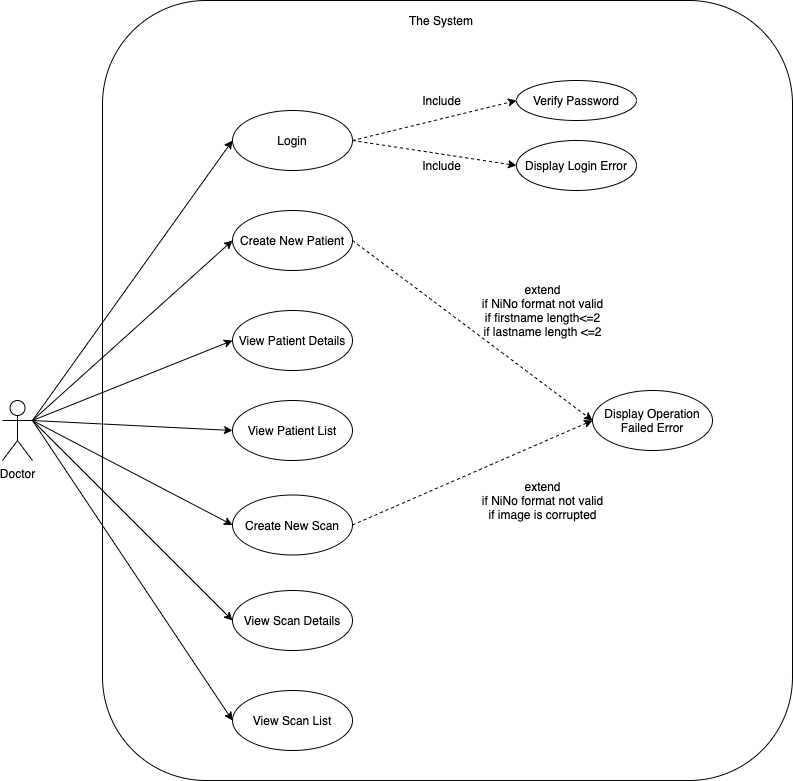
\includegraphics[scale=0.5]{figures/use-case}
				\fi
			\end{figure}
	\section{Non Functional Requirements}
		\label{non-functional-requirements}
		Nonfunctional requirements are the properties of the system; an comprehensive list of the agreed nonfuctional requirements is given below
		\begin{itemize}
			\item The system must be secure, as it handles the personal information of the patients
			\item The system should be reliable, as downtimes are affecting the hospital's performance 
			\item The system should be able to complete a prediction scan in a reasonable amount of time(1-10 mins)
		\end{itemize}
		



    \chapter{Entity Relation Analysis}
	\section{Introduction}
	After the requirements have been set. We need to translate them into workable relational entities in order to be able to modeled through a classical
	relational database system (RDBMS).
	\section{Entities}
	We will start our exploration by defining our entities for this project.
	\subsection{Scan}
	A scan is the result of an ultrasound scan performed in a specific patient(see [\ref{patient-definition})]. A scan entity has certain attributes
	\begin{center}
		\begin{tabular}{ |c|c| } 
			\hline
			Image & The image produced by the ultrasound scan. 360x560 pixels\\
			Prediction & The result of the prediction algorithm. Acceptable Values = {Maligrant, Benign}  \\
			Results & The logs of the algorithm performed the prediction, Optional \\
			Algorithm & The algorithm used to perform the prediction. Acceptable Values = {SVC,RES} \\
			Token& The scan identifier across the application services. token type is UUID [\cite{rfc4122}] \\
			\hline
		\end{tabular}
	\end{center}
	\subsection{Patient}
	\label{patient-definition}
	A patient is a physical person that is suspected to have a thuroid nodule. A person may have 0 up to n scans, where n is the theoretical
	maximum number of records(no limit is enforced by the database or the application). A patient has characteristics explaned below
	\begin{center}
		\begin{tabular}{ |c|c| } 
			\hline
			First Name & The first name of the patient.\\
			Last Name & The last name of the patient \\
			NiNo & The National Insurance Number(NiNo) of the patient \\
			Enrolled Date & The Date that the patient was registered in the system \\
			Ascosiate Doctor& The Doctor identification number, handling the case of the patient(see \ref{doctor-definition}) \\
			Comments& The Doctors(see \ref{doctor-definition}) comments for the particular patient\\
			\hline
		\end{tabular}
	\end{center}
	\subsection{Doctor}
	\label{doctor-definition}
	A doctor is a physical person with access on the system. Is the end-user of the system and has rights of uploading ultrasound image
	scans and retrieve predictions for those scans. It can also provide feedback to the system for a given prediction to be used for 
	further research and develepoment. A doctor has specific characteristics presented below.
	\begin{center}
		\begin{tabular}{ |c|c| } 
			\hline
			Username & Plain-text username\\
			Password & MD5 Hashed[\cite{rfc1321}] and salted[\cite{MANBER1996171}] password \\
			First Name & National Insurance Number[\cite{nino-format}] \\
			Last Name & The date that the patient was registered in the system \\
			Title& The title of the doctor.\\
			Enrolled Date& The date and time of the user enrolled to the system\\
			Last Seen& The date and time of last login of the user \\
			Online Status& The status of the user, acceptable values are Connected,Not Connected \\
			Tasks& The number of scans uploaded by the user \\
			\hline
		\end{tabular}
	\end{center}
	\subsection{Notification}
	\label{notification-definition}
	A notification is a short message from the system to the end-user(The doctor). Its sole purpose is to inform the user about
	various events that may interest the end-user. An example of this may be that the scan results for a given scan task are ready 
	to view. A notification has specific characteristics witch are displayed and explained below.
	\begin{center}
		\begin{tabular}{ |c|c| } 
			\hline
			Message & The message in question\\
			Ascosiated Doctor & The receipient doctor identification number \\
			Created Date & The Date and Time where the event in question where happened\\
			\hline
		\end{tabular}
	\end{center}
	\section{Entity Relations}
	The aforementioned entities have well defined relations. An exhaustive list is given below
	\begin{itemize}
		\item A doctor has many patients (1 - $\infty$)
		\item A doctor has many notifications(1 - $\infty$)
		\item A Patient has many Scans(1 - $\infty$)
	\end{itemize}
	A above relations can be summarized in the following E-R\footnote{Entity-Relation} Diagram
	\begin{figure}[H]
		\iftrue
		\centering
		\caption{Entity-Relation Diagram}
		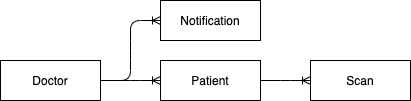
\includegraphics[scale=0.5]{figures/Entity-Relation-Fig}
		\fi
	\end{figure}



    \chapter{Users Perspective}
\label{users_perspective}
	\section{Introduction}
		In this section, we will start our exploration of the application and its features. As the nature of the requirements of this
		the system is complicated, unavoidably the system will be complex as well. Taking this into consideration, we will follow a natural top-to-bottom
		approach explaining its internals, starting as end-users and seeing the system as a black box. In this section, we will analyze its 
		functionality from the user's perspective. This section may also serve as an instruction manual for the end-user as it contains everything needed
		for an inexperienced user to start working with the software.
	\section{Login and Authentication}
		\begin{figure}[H]
			\iftrue
			\centering
			\caption{Login Screen}
			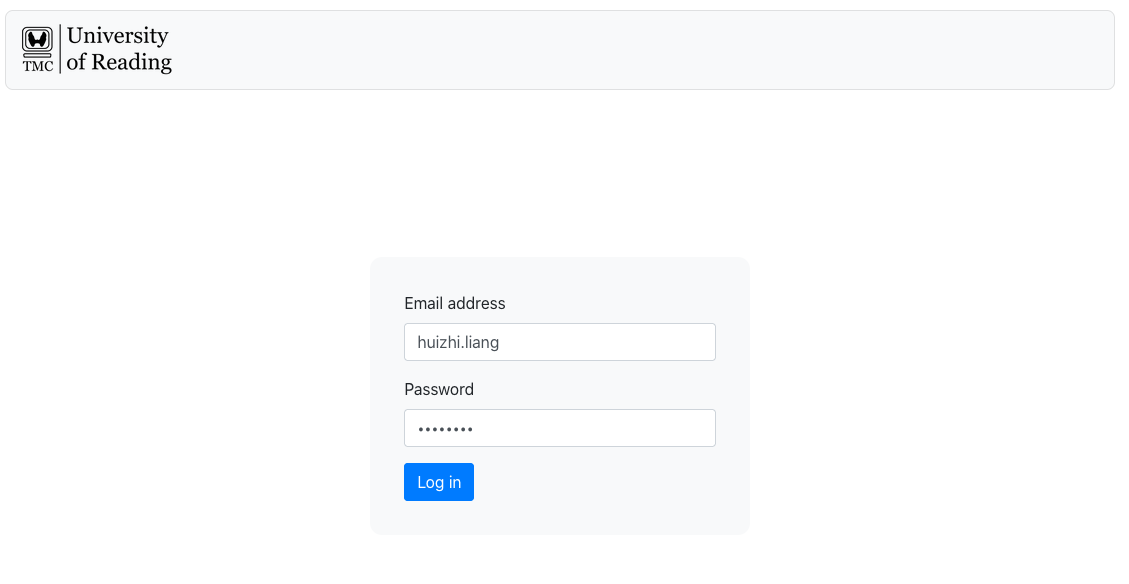
\includegraphics[scale=0.3]{figures/login}
			\fi
		\end{figure}
		The login screen is the first screen that our end-users will encounter. Here a username and a password is required to be given by the 
		user to log in. The Credentials of the user remain encrypted during the process of login, as the system utilizes an HTTPS[\cite{rfc2818}] 
		protocol for its connection, this is essential for the first non-functional requirement about security (paragraph \ref{non-functional-requirements}).
		An end-user may request a username and the password by the system administrator or the NOC\footnote{Network Operations Center} of the hospital.
	\section{Home}
		\begin{figure}[H]
			\iftrue
			\centering
			\caption{Home Screen}
			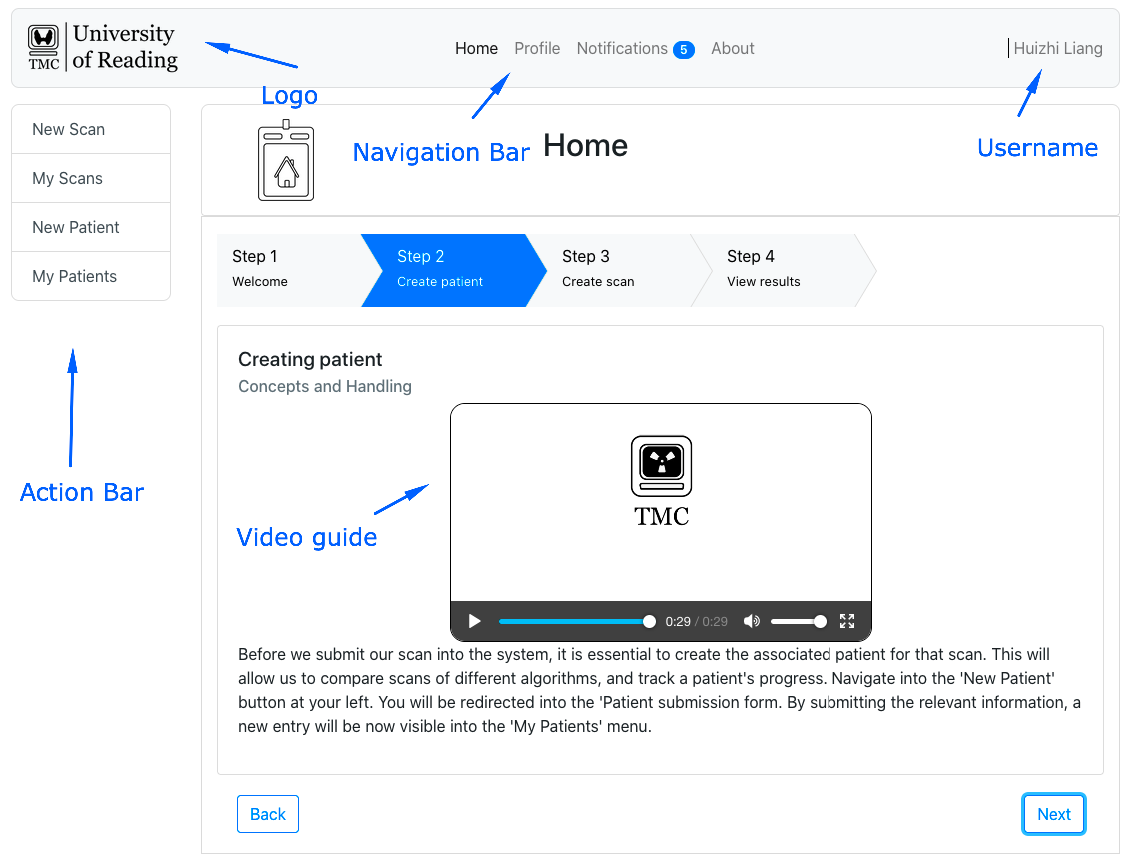
\includegraphics[scale=0.3]{figures/home}
			\fi
		\end{figure}
		After the login process is completed. The user encounters the 'home screen. From here, it is possible to navigate to the features of the software
		as well as learn about how the software can be utilized through detailed guides and videos. The UI/UX\footnote{User Interface-User Expieriance} 
		has been designed to be as user-friendly as possible. Some areas of interest are given below.
		\begin{center}
			\begin{tabular}{ |c|c| } 
				\hline
				Action bar & The Actions that can be performed using the software can be accesed from here.\\
				Navigation bar & General information and notification bar. \\
				\hline
			\end{tabular}
		\end{center}
	\section{Navigation bar}
		In this section, we will briefly look at the options under the Navigation bar.
		\subsection{Profile}
			\label{profile-screen}
			\begin{figure}[H]
				\iftrue
				\centering
				\caption{Profile}
				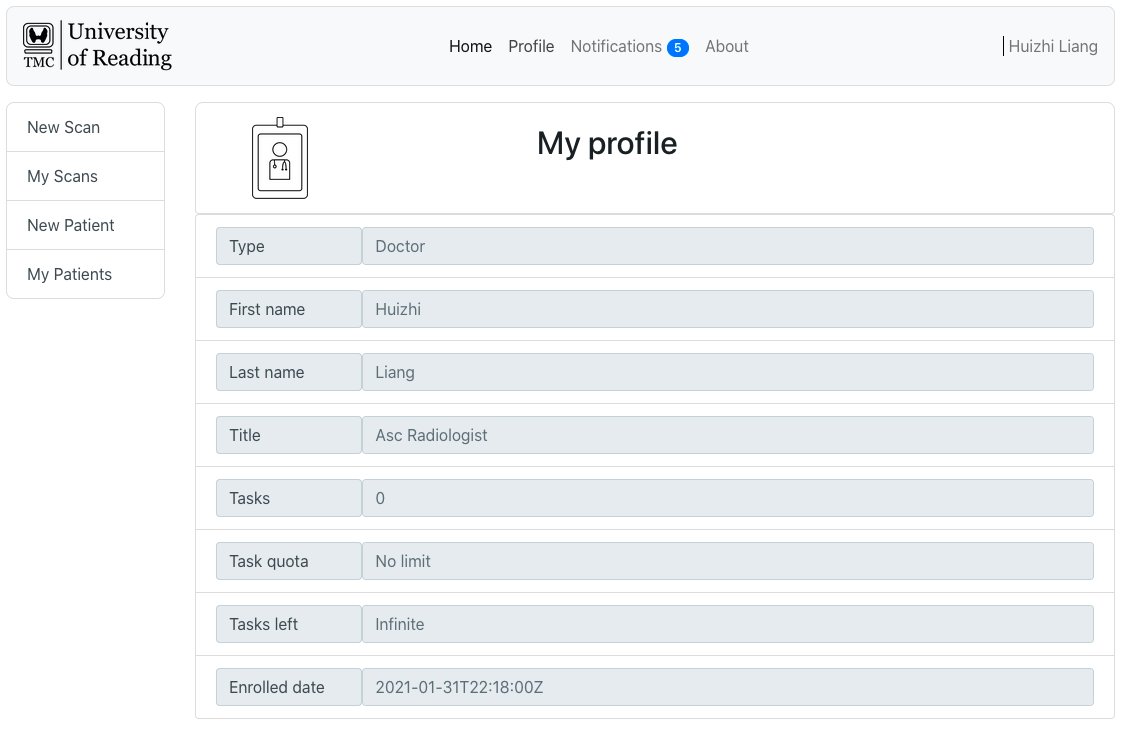
\includegraphics[scale=0.3]{figures/profile}
				\fi
			\end{figure}
			In the profile section, the user can see its associated information, saved on the registration date. 
			The information for security reasons cannot be altered by the user itself, but only after a request to 
			the system administrator or NOC\footnote{Network Operations Center} of the hospital.
		\subsection{Notifications}
			\label{notification-screen}
			\begin{figure}[H]
				\iftrue
				\centering
				\caption{Notifications}
				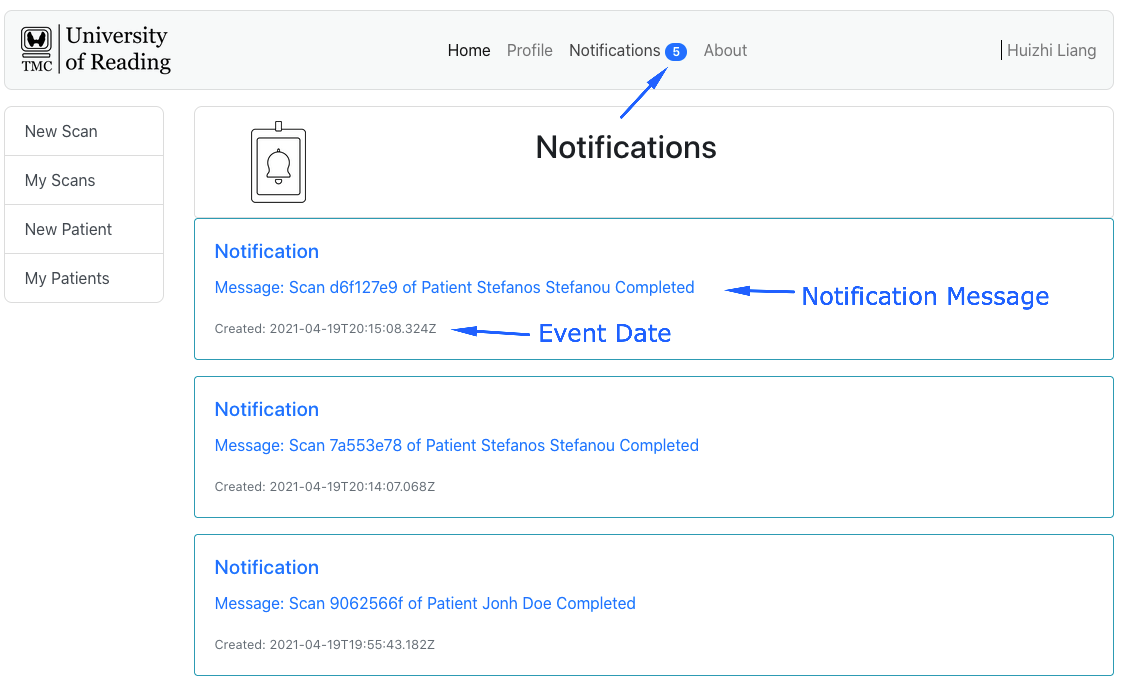
\includegraphics[scale=0.3]{figures/notifications}
				\fi
			\end{figure}
			In the notification section, helpful information about events that may interest the end-user can be found, 
			such as the fact that uploaded scan results are ready to view. 
		\subsection{About}
			\begin{figure}[H]
				\iftrue
				\centering
				\caption{About}
				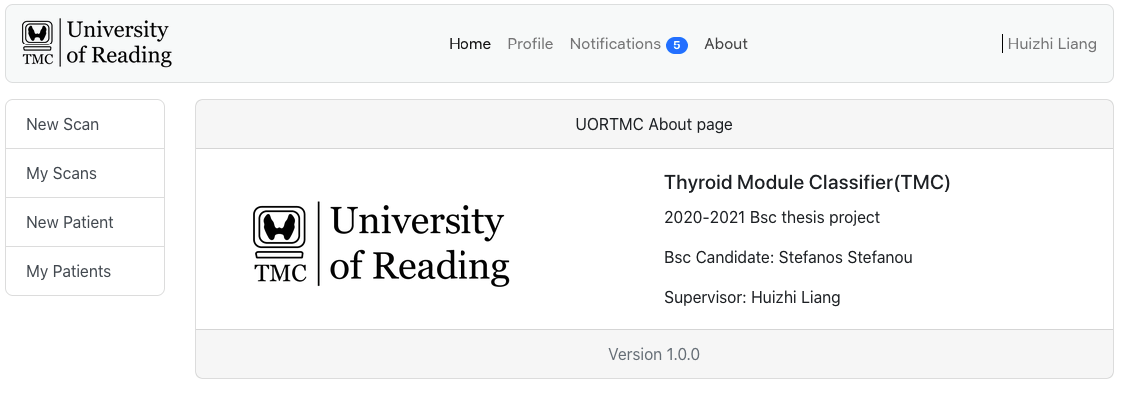
\includegraphics[scale=0.3]{figures/about}
				\fi
			\end{figure}
			From here, a user may found helpful information about the software, such as the current version.
	\section{Action Bar}
		In this section, we will briefly look at the options under the Action Bar.
		\subsection{My Patients}
			\label{my-patients}
			\begin{figure}[H]
				\iftrue
				\centering
				\caption{Patients List}
				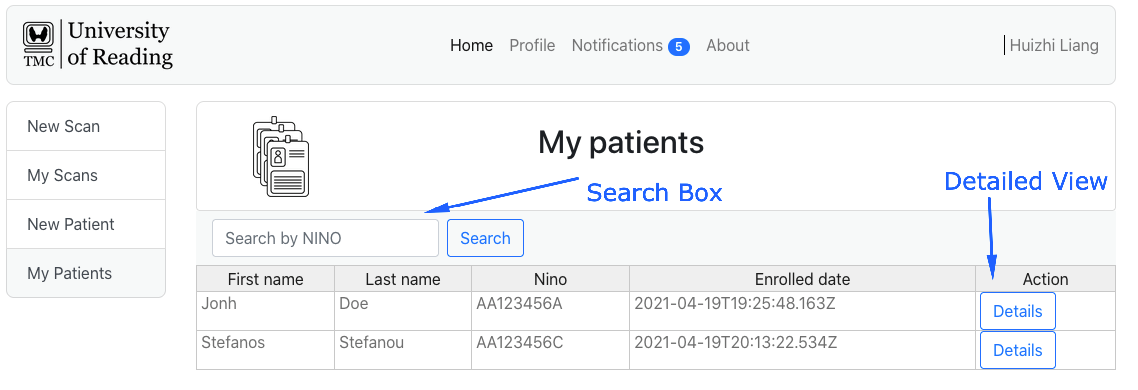
\includegraphics[scale=0.3]{figures/mypatients}
				\fi
			\end{figure}
			This page will show us a list of the currently registered patients. Each end-user(doctor) may only see its 
			patients and not others. The end-user can search the list based on NiNo[\cite{nino-format}] of the given 
			patient for convenience. The end-user can also view the details of a given patient and record various 
			notes/comments for that patient by clicking the 'Details' button on his selected patient, as seen below. 
			Finally, clicking the button 'View Scans' can see the specific patient history of uploaded scans.
			\begin{figure}[H]
				\iftrue
				\centering
				\caption{Patient Details}
				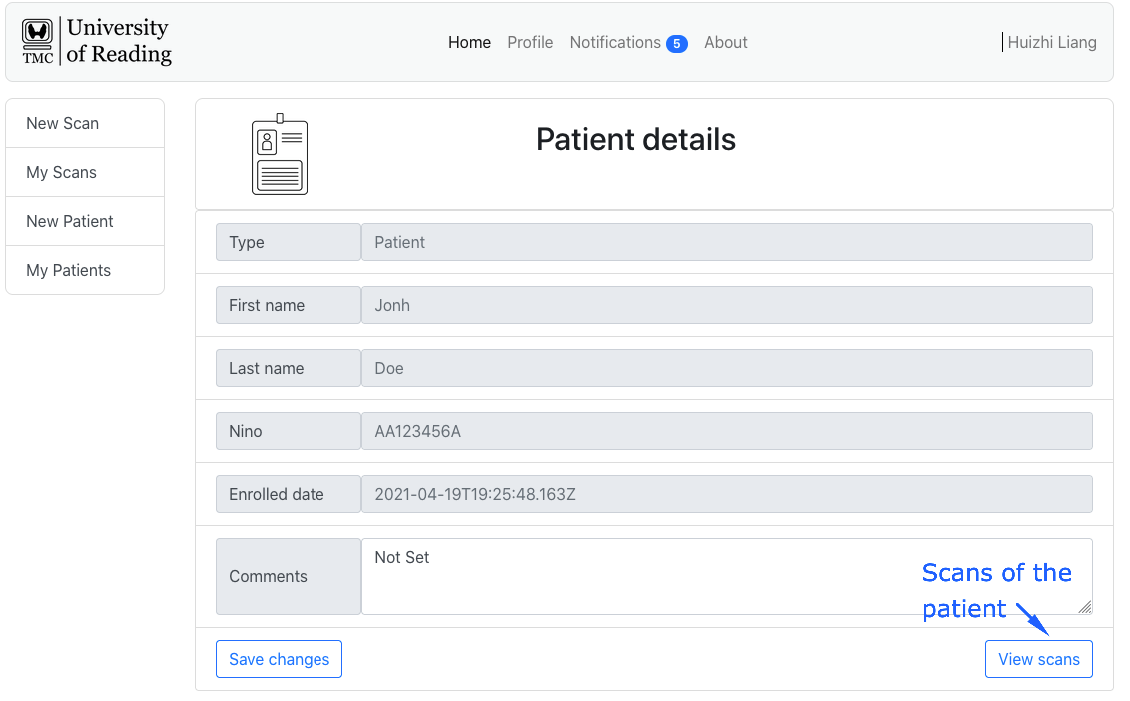
\includegraphics[scale=0.3]{figures/mypatients2}
				\fi
			\end{figure}
		\subsection{New Patient}
			\label{patient-submission}
			\begin{figure}[H]
				\iftrue
				\centering
				\caption{New Patient}
				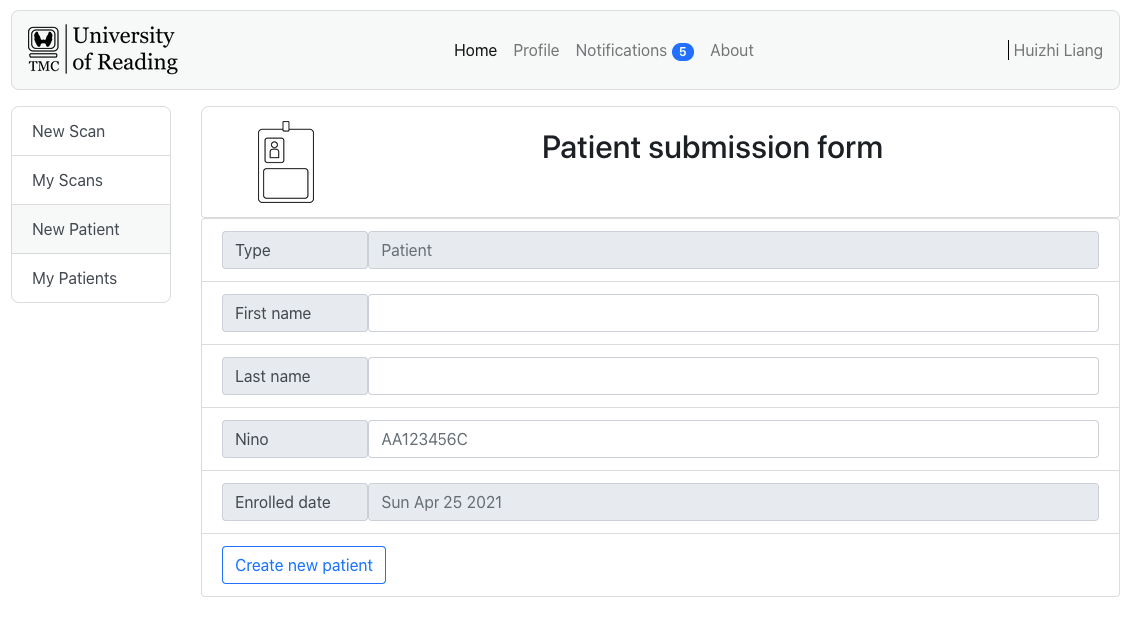
\includegraphics[scale=0.3]{figures/newpatient}
				\fi
			\end{figure}
			By clicking the 'New Patient' action on Action Bar, the user can register a new patient on the system. The following conditions need to 
			be met for the operation to be successful.
			\begin{itemize}
				\item First name length should be more than 2 characters, encoded as UTF-8[\cite{rfc3629}]
				\item Last name length should be more than 2 characters, encoded as UTF-8[\cite{rfc3629}]
				\item NiNo should be at standard format [\cite{nino-format}], encoded as UTF-8[\cite{rfc3629}]
			\end{itemize}
			Failing to fulfill these constraints should lead to an error, as shown below.
			\begin{figure}[H]
				\iftrue
				\centering
					\caption{New Patient Error}
				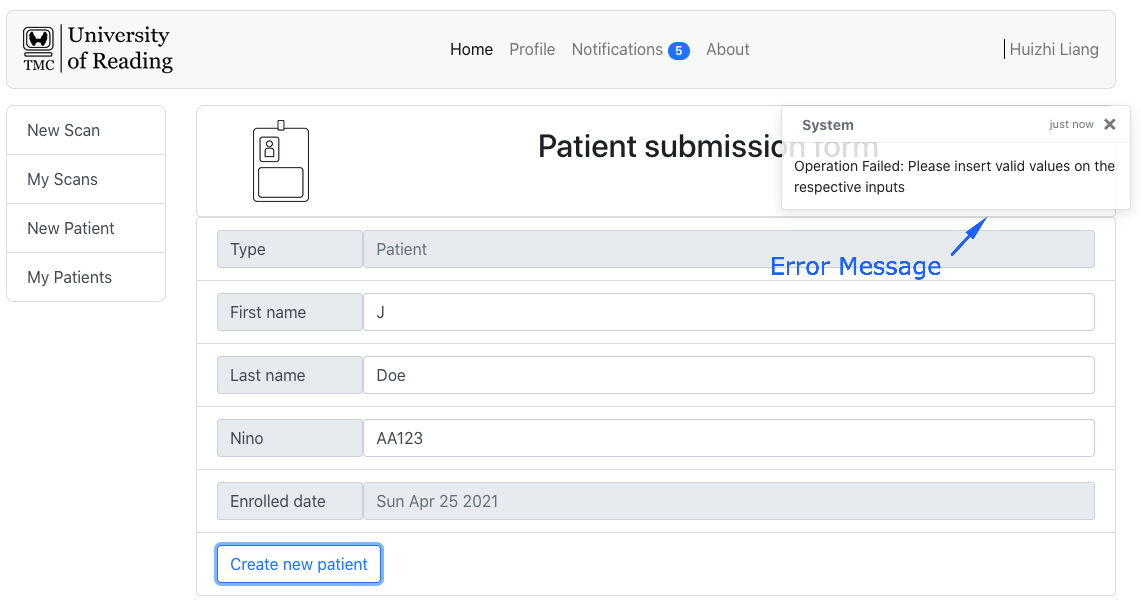
\includegraphics[scale=0.3]{figures/newpatient-error}
				\fi
			\end{figure}
		\subsection{My Scans}
			\label{my-scans}
			\begin{figure}[H]
				\iftrue
				\centering
				\caption{My Scans}
				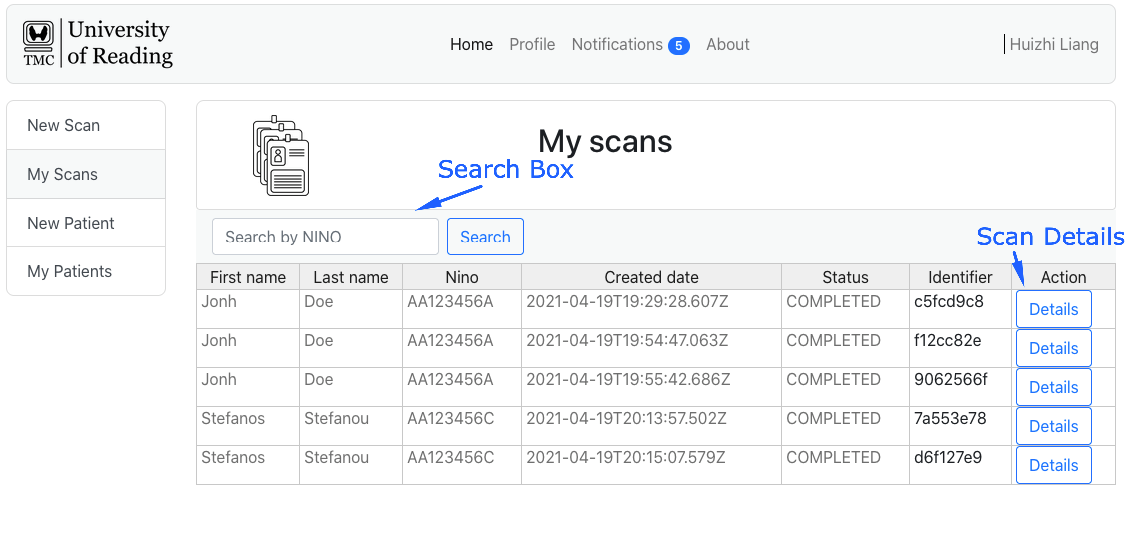
\includegraphics[scale=0.3]{figures/myscans}
				\fi
			\end{figure}
			'MyScans' are a complete list with all submitted scans for a given end-user. 
			The user can search for the scans of a specific patient by using the search box and viewing the 
			scan results (if a given scan is complete) by clicking the 'Details' button of the scan in question.
			\begin{figure}[H]
				\iftrue
				\centering
				\caption{Scan results}
				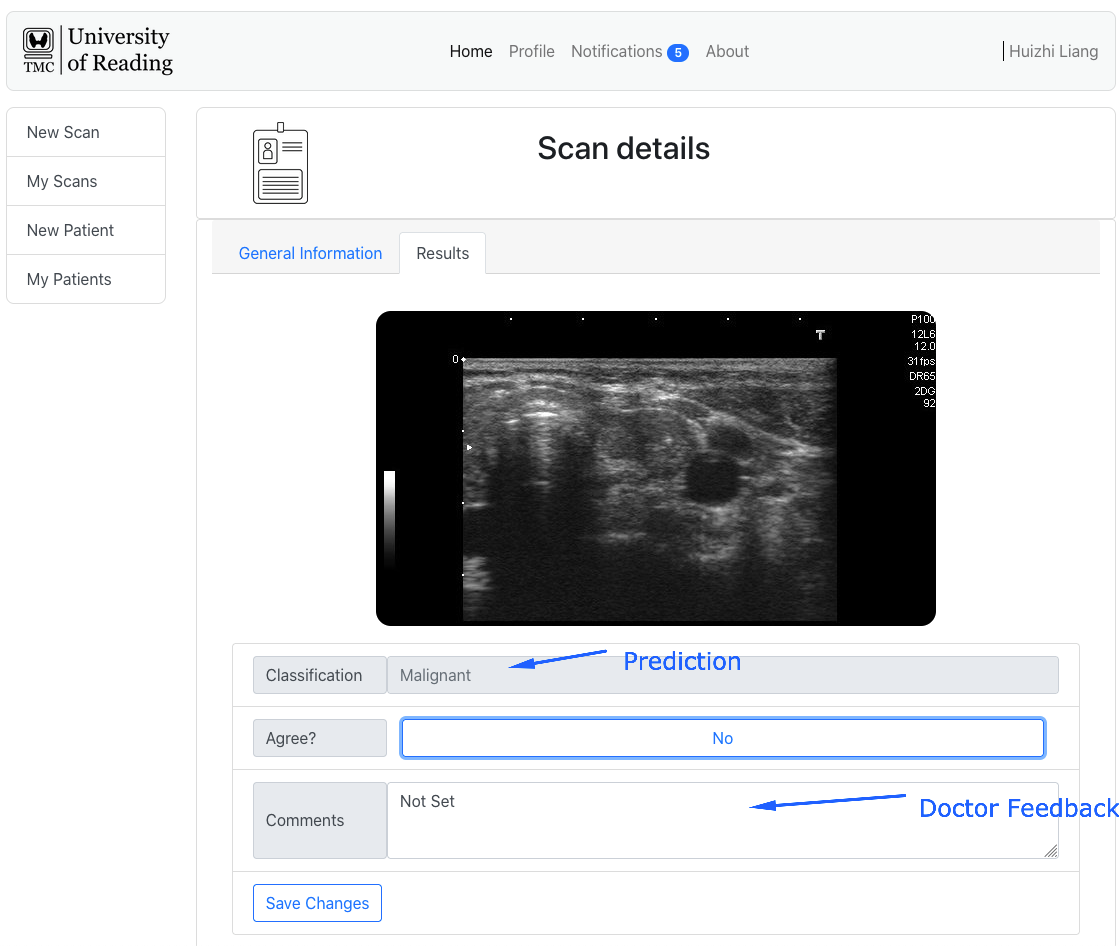
\includegraphics[scale=0.3]{figures/myscans-details}
				\fi
			\end{figure}
		\subsection{New Scan}
			\label{new-scan}
			\begin{figure}[H]
				\iftrue
				\centering
				\caption{New Scan}
				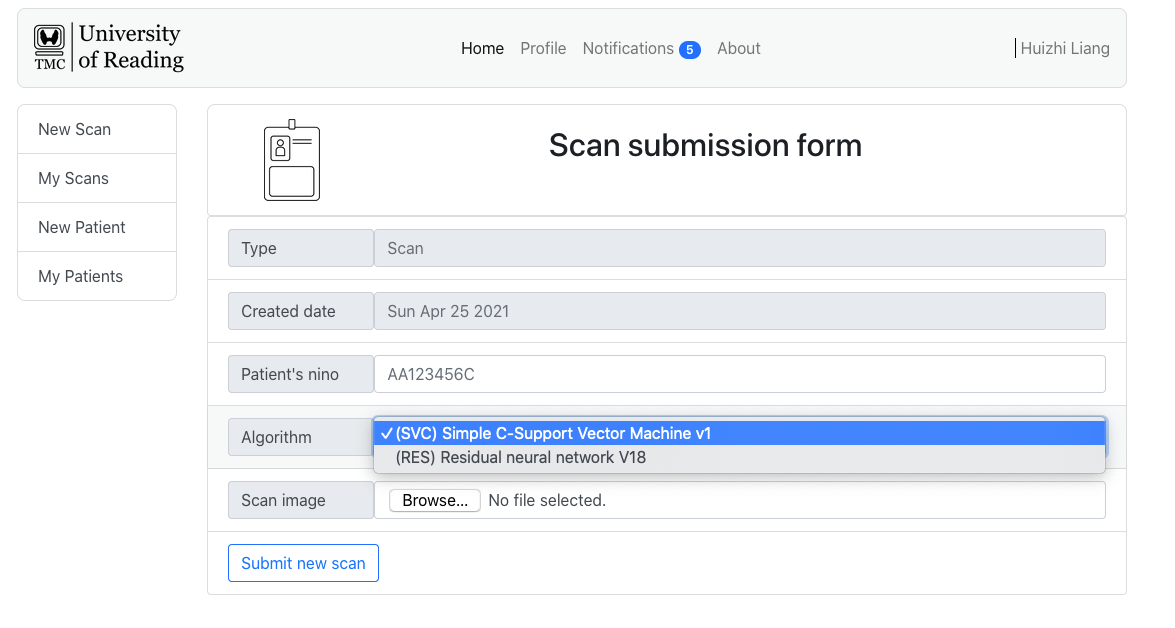
\includegraphics[scale=0.3]{figures/newscan}
				\fi
			\end{figure}
			By clicking the 'New Scan' action, the user is redirected into the scan submission form. Here it is possible to 
			submit a new ultrasound image for a given patient. The user can also select the algorithm for performing the 
			classification (see \ref{prediction-process}). The operation to be completed should meet the following criteria.
			\begin{itemize}
				\item Patients Nino should be in standard format[\cite{nino-format}] and encoded as UTF-8[\cite{rfc3629}]
				\item Scan Image should be a ISO/IEC 10918-1/JPEG[\cite{jpeg-iso10918-1}] format with 360x560 resolution. The image name
				should be encoded as UTF-8[\cite{rfc3629}]
			\end{itemize}
			Failing to fulfill these constraints should lead to an error, as shown below.
			\begin{figure}[H]
				\iftrue
				\centering
				\caption{Invalig image format (PNG) error}
				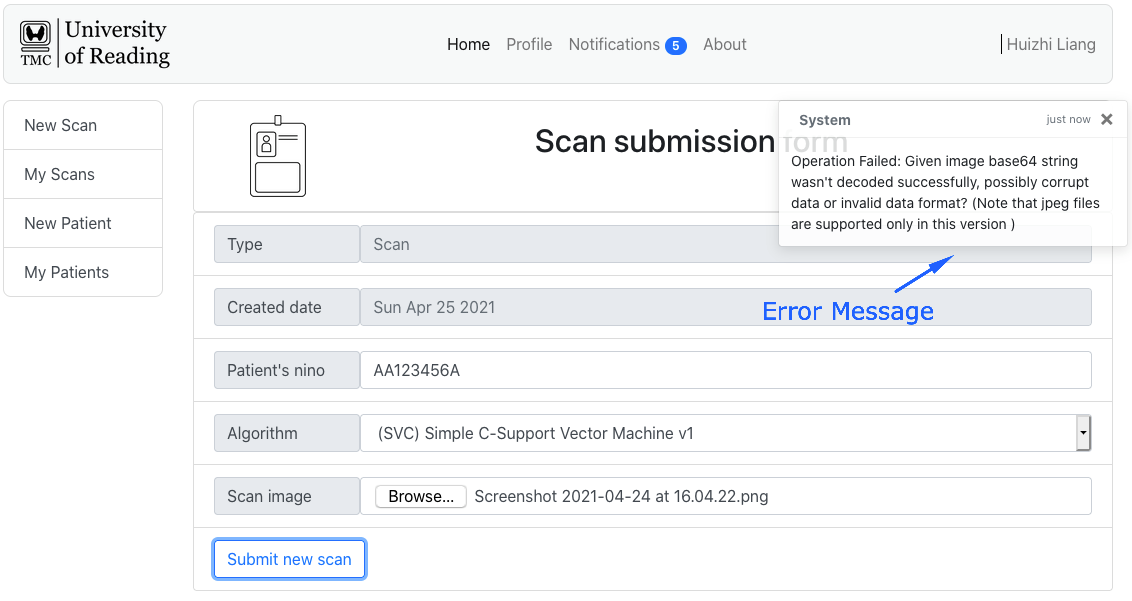
\includegraphics[scale=0.3]{figures/newscan-error}
				\fi
			\end{figure}
			
			
			
			
			
			
			
		
	




    \chapter{System Architecture}
	\label{architecture}
	In this chapter, we will introduce the architecture of our system, explaining the essential elements that it is 
	composed of and their interactions.
	\section{Overview}
		In the section \ref{non-functional-requirements} we discussed the non-functional requirements of this application. Two 
		of the most important ones were security and performance. These requirements heavily influenced the design decisions 
		of this project, leading to the microservice-inspired architecture [\cite{newman_2020}]shown below.
		\begin{figure}[H]
			\iftrue
			\caption{Simplified Architectural Diagram}
			\centering
			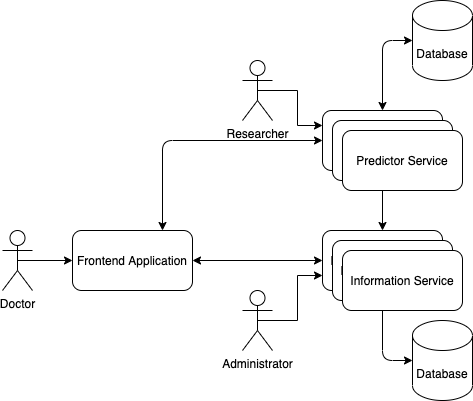
\includegraphics[scale=0.5]{figures/system-architecture}
			\fi
		\end{figure}
		Microservice pattern[\cite{newman_2020}] tries to decrease complexity and increase safety by splitting the internal logic 
		of a system into several components called 'Microservices'. Each microservice is essentially a server that handles a small 
		portion of the systems logic. As opposed to the  monolithic services, microservices have a number of advantages that made 
		them ideal for the requirements of this project such as.
		\begin{itemize}
			\item Highly maintainable and testable code
			\item Loosely coupled logic
			\item Independently deployable services
			\item No single point of failure
			\item Flexible scaleability factor
			\item Enchanced security
		\end{itemize}
		\subsection{Maintainability}
			By implementing our system using microservices[\cite{newman_2020}], we effectively separate the complex 
			logic of our system into different services. This separation of complexity leads to several elementary and 
			easily testable and maintainable entities. This brings down the maintenance costs.
		\subsection{Loosely coupled logic}
			Microservices ideally are loosely coupled. That means that changes tend to remain local to one microservice and do 
			not span multiple ones. In case that the requirements change and new features are needed, the features will not affect 
			a significant part of the code. This translates more negligible probability of occurring bugs and errors.
		\subsection{Indepedently deployable services}
			Using microservices gives us the advantage of deploying changes independently on the system, only on services that we need.
			This translates to fewer downtimes due to maintenance. An example of this will be a potential deployment of a new
			algorithm on the Prediction service. During the deployment of the new version of the Prediction service the system 
			will be unable to perform predictions, but the rest of the functionality will be unaffected as it lies under a different 
			microservice. With a monolith approach(all functionality in a single service), this would not be possible.
		\subsection{No single point of failure}
			Using microservices, we ensure that it will not propagate to the whole system when a failure occurs. In the hypothetical 
			scenario of a failure in the Prediction service, the rest of the system's functionality will remain intact during the 
			incident. This scenario with a monolithic architecture will bring the whole application into an unusable state.
		\subsection{Flexible scaleability factor}
			This is not sorely a feature of microservices but a combined feature brought by some additional design choices 
			from within the code itself. Both of the services are implemented using the actor model [\cite{hewitt2015actor}]. 
			The actor model allows, in combination with the microservice model, our services to act as a distributed system with 
			multiple nodes; this allows us to scale different services when demand changes dynamically and automatically, ensuring 
			the performance non-functional requirement we set back in \ref{non-functional-requirements}. An example of this can be 
			when multiple users simultaneously use the most advanced and CPU-Intensive algorithm, the ResNet(see \ref{prediction-process}). 
			If the system determines that the load is beyond some threshold, it can spin multiple instances of the same service. 
			The instances will coordinate themselfs automatically and split the work that needs to be done into equal amounts, 
			reducing the response time. This is implemented using the Heroku-autoscale feature and will be discussed in chapter \ref{backend}
		\subsection{Enchanced security}
			Having multiple and distinct microservice enhances security, as the malicious compromise of one microservice does not
			 imply the compromise of the whole system. In the hypothetical scenario of a malicious attacker may breach the 
			 Prediction Service, then the data of the Prediction Service will be at risk, but not the data from the Information 
			 System and vice versa.
	\section{Frontend Web App}
		The Frontend component has the responsibility of being the edge in our system.
		\begin{figure}[H]
			\iftrue
			\caption{Frontend Application}
			\centering
			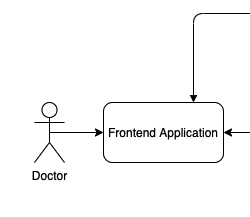
\includegraphics[scale=0.5]{figures/frontend}
			\fi
		\end{figure}
		Every action from our end-users, will be channeled through the frontend application. Our frontend is a web-based application(for 
		more information please see \ref{frontend}) and handles the application infastructure via a well designed stateful[\cite{session-rfc6265}],
		Json-based[\cite{json-rfc7159}] Https[\cite{rfc2818}] RESTFull[\cite{restful-rfc7231}]
		protocol (for more information please see chapter \ref{API}).
	\section{Backend}
		The backend services are the backbone of our application. They handle all the logic behind the application, from the saving 
		and retrieval of patients, scans, images, and notifications, to the prediction and classification of the ultrasound images. 
		There are two services with distinct areas of interest and different purposes, the Information Backend(also known as 
		'Information Service' to the simplified diagrams) and Task Backend(Also known as Predictor Service).
		\subsection{Information Backend}
			\begin{figure}[H]
				\iftrue
				\caption{Information Service}
				\centering
				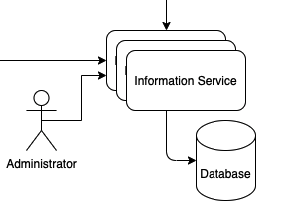
\includegraphics[scale=0.5]{figures/infobe}
				\fi
			\end{figure}
			The Information Backend has the responsibility to perform all the logic apart from the prediction itself. It
			 includes the functionality of keeping the associations of Patients, Scans, and the information composing those 
			 entities. It also includes the notification system and authentication services. Finally, it includes a small 
			 application for use by the NOC\footnote{Network operations center}  for administrator purposes.
		\subsection{Task Backend}
			\begin{figure}[H]
				\iftrue
				\caption{Predictor Service}
				\centering
				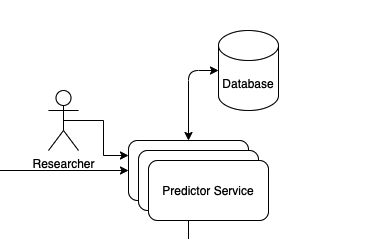
\includegraphics[scale=0.5]{figures/taskbe}
				\fi
			\end{figure}
			The Task Backend has the responsibility of performing the predictions based on the received ultrasound scan images. 
			After completing a prediction, Task Backend should communicate with Information Backend to inform the user about the 
			completion of the scan. Finally, it includes a small application for use by the researcher to gather the data and the 
			feedback from the end-users.
	
		
				
					
			
		
	

    \chapter{The Administrators Perspective}
\label{admin_perspective}
	\section{Introduction}
		In this section, we will briefly go through the application interface for the administrator of the system. 
		The administrator of the system has special rights and is assigned by the hospital that uses the software. 
		It needs to belong to the NOC\footnote{Network  Operations Center} of the hospital, and it is responsible for 
		the maintenance of the software in the DevOps Level.
		\begin{figure}[H]
			\iftrue
			\caption{Information Service}
			\centering
			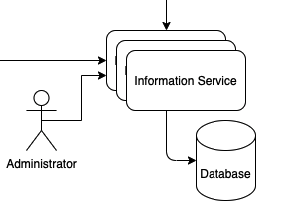
\includegraphics[scale=0.5]{figures/infobe}
			\fi
		\end{figure}
	\section{Administrator Panel}
		The administrator has special tools for maintaining the system and intervene in its internals, a special administrator panel that gives access to a 
		plethora of features that needs to be handled with care. 
		\begin{note}
			To connect to the administrator panel, we need to connect to the following addresses\\
			\begin{center}
				(if online) https://uortmc-infobe.herokuapp.com/admin/ \\
				(local machine )http://127.0.0.1:3001/admin
			\end{center}
			Please refer to the chapter \ref{cicd-versioning-deployment} and chapter \ref{start-stop-guide} for more details around how to connect.
		\end{note}
		\subsection{Admin Panel Login}
			\begin{figure}[H]
				\iftrue
				\caption{Administrator Panel}
				\centering
				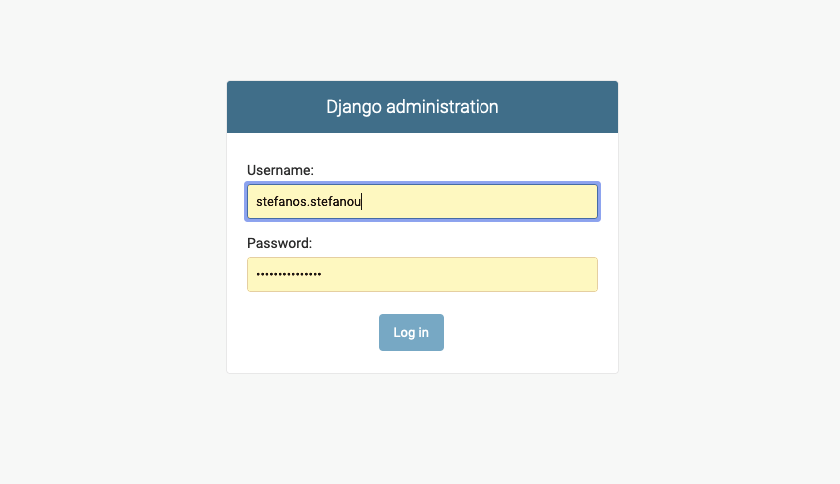
\includegraphics[scale=0.3]{figures/admin-panel-login}
				\fi
			\end{figure}
			The login screen is the first screen that an admin should encounter. The information transmitted into the Information Service
			is encrypted using HHTPS[\cite{rfc2818}] and transformed to an salted[\cite{MANBER1996171}] MD5 Hash[\cite{rfc1321}] for maximum 
			possible security.
		\subsection{Admin Panel Features}
			\begin{figure}[H]
				\iftrue
				\caption{Administrator Panel-Home}
				\centering
				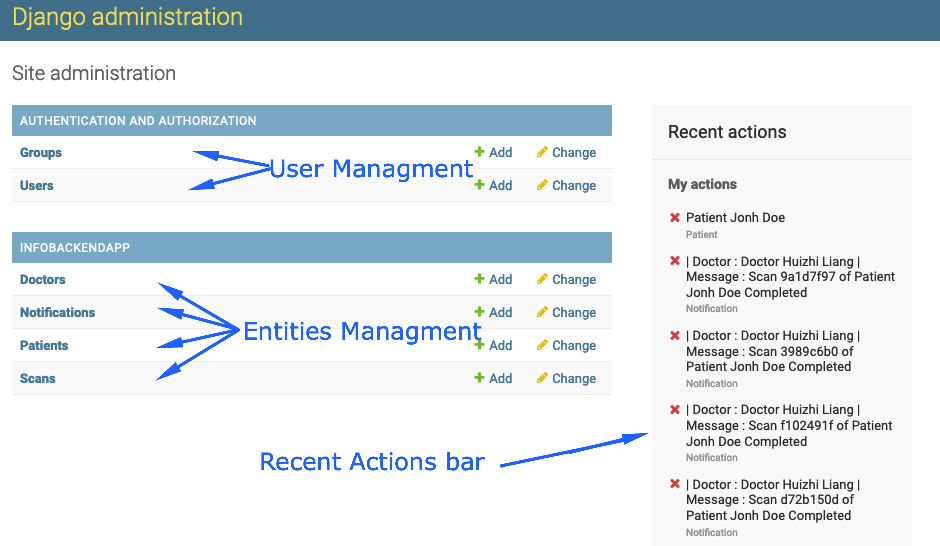
\includegraphics[scale=0.3]{figures/admin-panel-home}
				\fi
			\end{figure}
			After the login sequence is completed, the administrator will be redirected to the panel's home page; there, 
			it has available all the functionality needed to perform changes on the system. An administrator 
			has the right to alter the system's properties as well as the entity's attributes. We can add, alter and 
			delete entities at will, using the Entities Management.
			\begin{figure}[H]
				\iftrue
				\caption{Example deletion of a scan}
				\centering
				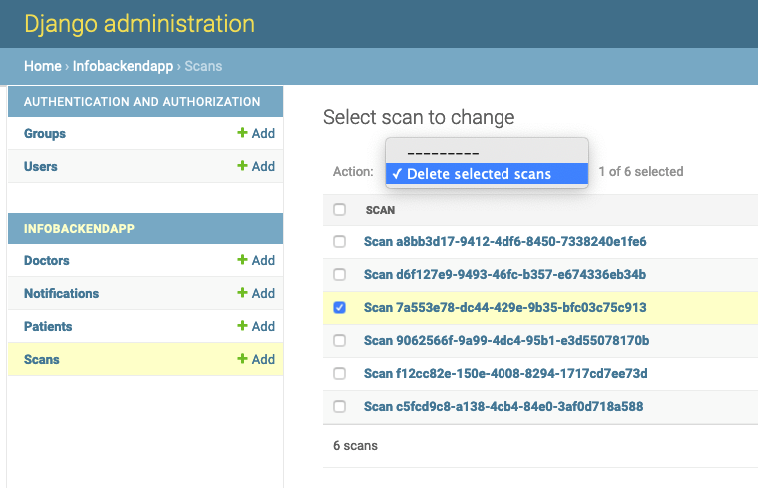
\includegraphics[scale=0.3]{figures/admin-panel-example-1}
				\fi
			\end{figure}
			\begin{figure}[H]
				\iftrue
				\caption{Example alteration of a patient}
				\centering
				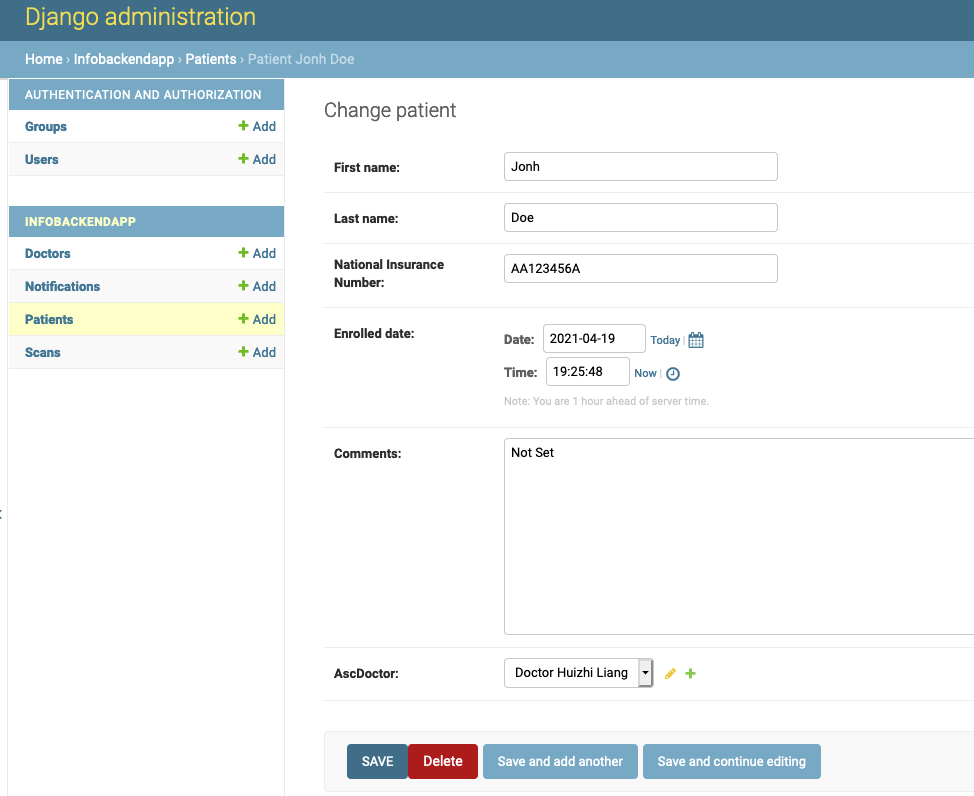
\includegraphics[scale=0.3]{figures/admin-panel-example-2}
				\fi
			\end{figure}
			
		
			
			
			
			
			
			
		
	




    \chapter{The Researchers Perspective}
\label{researchers_perspective}
	\section{Introduction}
		In this section, we will briefly look at the available features for the researcher of the project. 
		Every scientist working in prediction models for thyroid nodule classification may upload its algorithm 
		on the platform and receive helpful feedback about its performance using the Researcher panel explained below. 
		Visually the researcher's panel is nearly identical to the administrator panel explained in chapter 
		\ref{admin_perspective} but offers access to the different data than the administrator panel. This is done 
		to reduce costs and reuse the similar functionality developed for the administrator panel. The researcher panel 
		is provided by the Predictor Service(Task Backend).
		\begin{figure}[H]
			\iftrue
			\caption{Predictor Service}
			\centering
			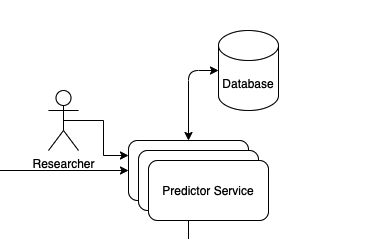
\includegraphics[scale=0.5]{figures/taskbe}
			\fi
		\end{figure}
	\section{Researcher Panel}
		The researcher panel provides an interface to the researcher to view its algorithm outputs and performance in an easy and user-friendly manner.
		\begin{note}
			To connect to the researcher panel, we need to connect to the following addresses\\
			\begin{center}
				(if online) https://uortmc-taskbe.herokuapp.com/admin/ \\
				(local machine )http://127.0.0.1:3002/admin
			\end{center}
			Please refer to the chapter \ref{cicd-versioning-deployment} and chapter \ref{start-stop-guide} for more details around how to connect.
		\end{note}
		\subsection{Login screen}
			\begin{figure}[H]
				\iftrue
				\caption{Researcher panel login screen}
				\centering
				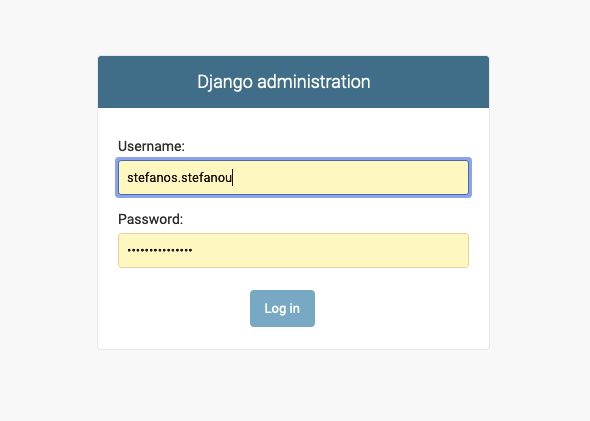
\includegraphics[scale=0.5]{figures/research-panel-login}
				\fi
			\end{figure}
			The login screen is the first screen that an researcher should encounter. The information transmitted into the Predictor
			Service is encrypted using HHTPS[\cite{rfc2818}] and transformed to an salted[\cite{MANBER1996171}] MD5 Hash[\cite{rfc1321}] 
			for maximum possible security. 
		\subsection{Researcher Panel Features}
			\begin{figure}[H]
				\iftrue
				\caption{Researcher Panel-Home}
				\centering
				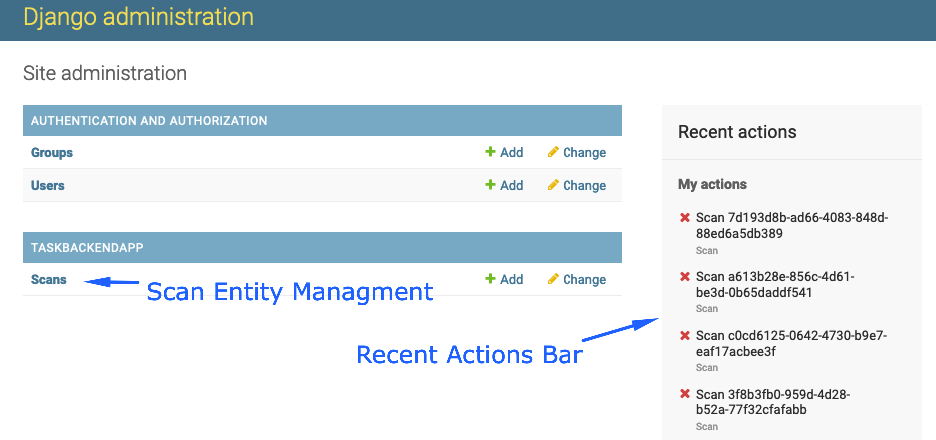
\includegraphics[scale=0.3]{figures/research-panel-home}
				\fi
			\end{figure}
			After the login sequence is completed, the researcher will be redirected to the panel's home page; there, 
			it has available all the functionality needed to perform debbuging into the algorithm under develepoment, such as 
			real-time logging capability. By selecting the scan in question can have access to the required information
			\begin{figure}[H]
				\iftrue
				\caption{Researcher Panel-List of scans}
				\centering
				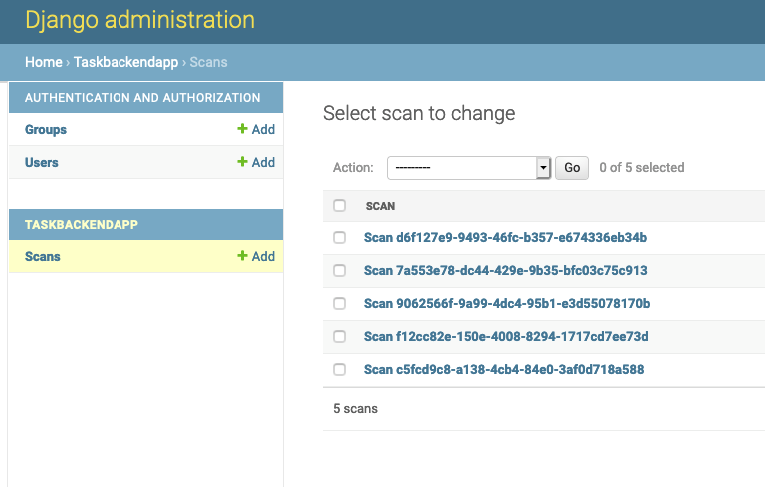
\includegraphics[scale=0.3]{figures/research-panel-scan-list}
				\fi
			\end{figure}
			\begin{figure}[H]
				\iftrue
				\caption{Researcher Panel-Scan Details Example}
				\centering
				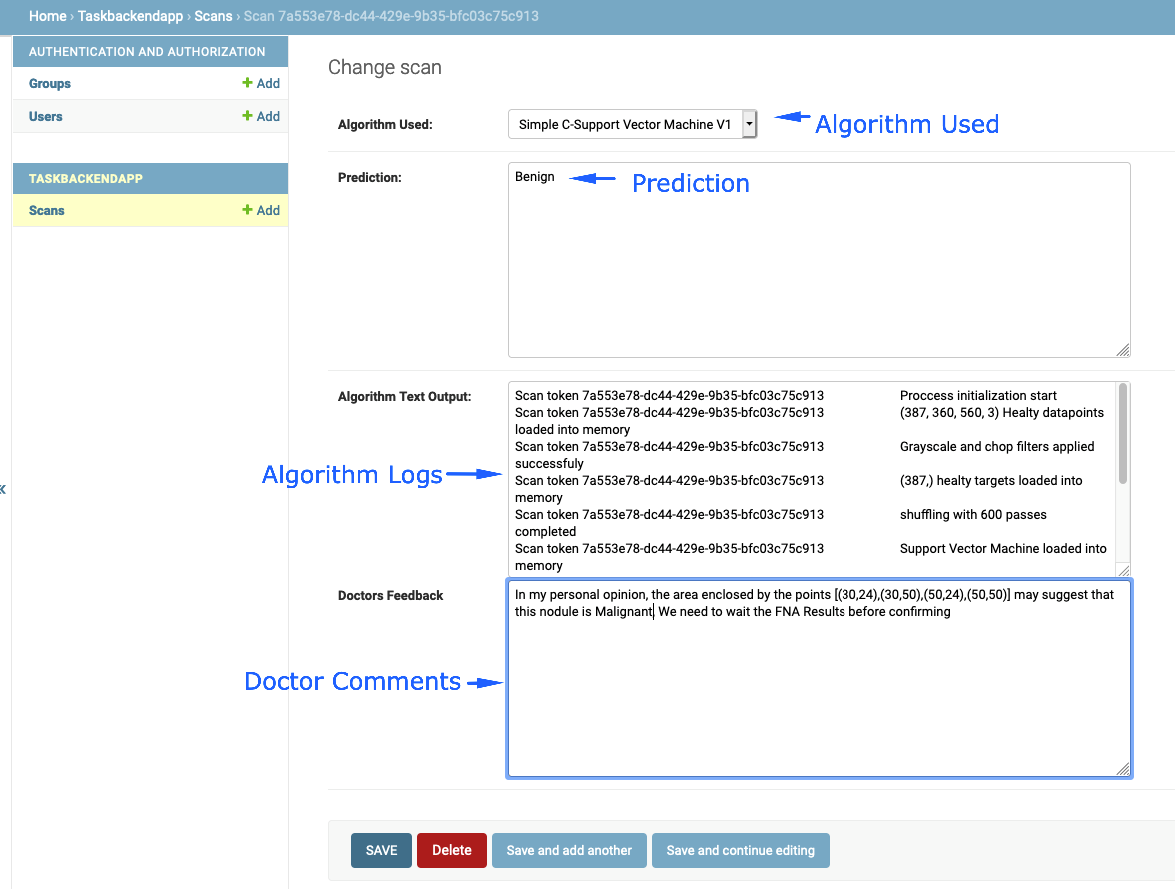
\includegraphics[scale=0.3]{figures/research-panel-scan-view}
				\fi
			\end{figure}
			The researcher then can improve the algorithm based on the feedback provided from the doctors, as well as to troubleshoot
			possible errors using the real-time logging capability.
			
			
			
			
		
		
		
			
			
			
			
			
		
	




    \chapter{The Frontend Application}
\label{frontend}
	\section{Introduction}
		\begin{figure}[H]
			\iftrue
			\caption{Frontend Application}
			\centering
			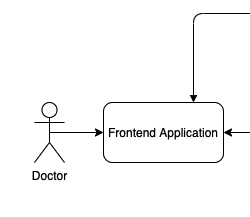
\includegraphics[scale=0.5]{figures/frontend}
			\fi
		\end{figure}
		In this chapter we will have a look at the technology stack, internals and points of interest of the frontend application. The
		frontend applications purpose is to serve as a visual middleware between the end-user (The Doctor) and the system itself. It 
		propagates the actions of the user into the system by using plain HTTPS Requests, via a stateful[\cite{session-rfc6265}],
		Json-based[\cite{json-rfc7159}] Https[\cite{rfc2818}] RESTFull[\cite{restful-rfc7231}]
		protocol (for more information please see chapter \ref{API}).
	\section{Technology Stack}
		The Frontend application uses the following frameworks and libraries
		\begin{itemize}
			\item React v18.0
			\item Boostrap v4
			\item Axios Requests
			\item Hansontable v8.3.2
		\end{itemize}
		\subsection{React}
			React.js is an javascript open-source framework for developing front-end applications. It is created by Facebook and 
			maintained by the open-source communinity as well as from some individual companies. It encourages the creation applicatios
			with well defined state and state transisions by composing lightweight and reusable UI Elements called 'Components'. The
			behaviour of the system is modelled strictly by events generated as a result of a state transision and the components should
			act accordingly. Our Frontend Application contains 13 indepedent components that communicate with each other by callbacks.
			An exchaustive list of the components is given below
			\begin{center}
				\begin{tabular}{ |c|c|c| } 
					\hline
					About & The About page &
\includegraphics[scale=0.2]{figures/component-about}\\
					About & The About page &
\includegraphics[scale=0.2]{figures/component-about}\\
					About & The About page &
\includegraphics[scale=0.2]{figures/component-about}\\
					About & The About page &
\includegraphics[scale=0.2]{figures/component-about}\\
					About & The About page &
\includegraphics[scale=0.2]{figures/component-about}\\
					About & The About page &
\includegraphics[scale=0.2]{figures/component-about}\\
					About & The About page &
\includegraphics[scale=0.2]{figures/component-about}\\
					About & The About page &
\includegraphics[scale=0.2]{figures/component-about}\\
					About & The About page &
\includegraphics[scale=0.2]{figures/component-about}\\
					About & The About page &
\includegraphics[scale=0.2]{figures/component-about}\\
					About & The About page &
\includegraphics[scale=0.2]{figures/component-about}\\
					About & The About page &
\includegraphics[scale=0.2]{figures/component-about}\\
					About & The About page &
\includegraphics[scale=0.2]{figures/component-about}\\
					\hline
				\end{tabular}
			\end{center}
			
    \chapter{The Application Programming Interface}
\label{API}
	\section{Introduction}
		In this section we will briefly discuss the commnunication protocol used by the application to its internal components. The protocol used as mentioned
		already in the previous chapters, is a designed stateful[\cite{session-rfc6265}], Json-based[\cite{json-rfc7159}] Https[\cite{rfc2818}] RESTFull[\cite{restful-rfc7231}]
		protocol. Let us explain briefly what those techical terms mean.
		\subsection{Stateful Protocol}
			Stateful protocol[\cite{session-rfc6265}] is a protocol capable of recognising and distinquishing between the different requests made by the same host machine. 
			In our application this is essential because the authentication functionality would be impossible otherwise. An authenticated user is 
			always ascosiated with a sessionID. The sessionID[\cite{sessionID-rfc7329}] is a character string that is returned after the authentication is 
			complete and should be attached to every subsequent request for user authentication to work. Our application protocol uses the cookie mechanism
			to attach the sessionID to every request, ensuring that the Services will recognise the sender. The following image provides an example
			\begin{figure}[H]
				\iftrue
				\caption{Session ID Attached to Notifications Request, captured using Firefox-Tools}
				\centering
				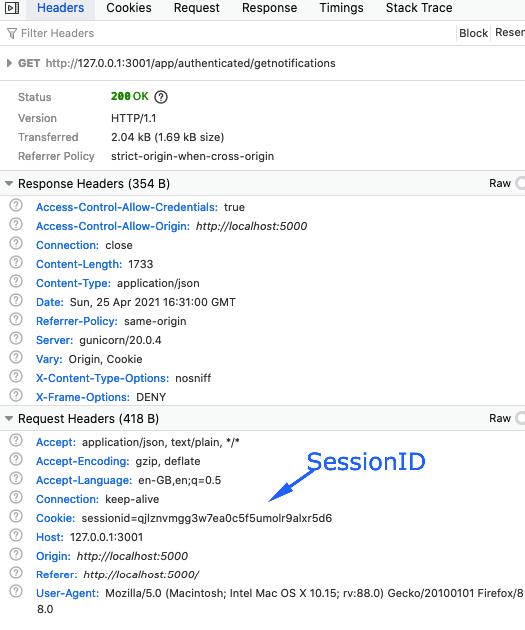
\includegraphics[scale=0.3]{figures/sessionID}
				\fi
			\end{figure} 
			Here, the Session ID is attached to a request from the Frontend Application into the Information Service, for the retrieval of new notifications
		\subsection{Json}
			The JavaScript Object Notation (or JSON) Data Interchange Format[\cite{json-rfc7159}] is a text-based, lightweight, human-readable language-indepedent
			data exchange format. We use JSON extensively to design our communication protocol, mainly because of his widely adopted use and availability of
			decoders. Additionally, both languages involved in the data transaction(javascript for the frontend, python for the backend services) are supporting
			JSON natively.
			\begin{figure}[H]
				\iftrue
				\caption{Capturing the Information service's JSON-Based responce using Postman}
				\centering
				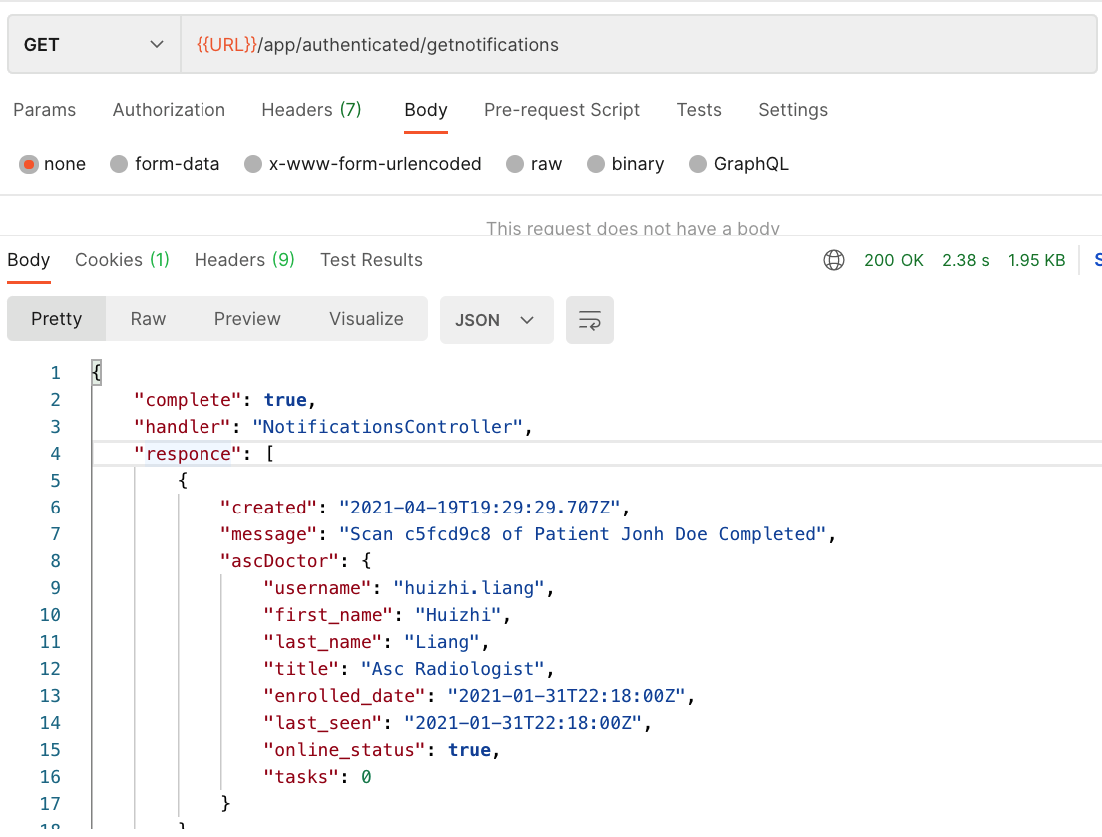
\includegraphics[scale=0.3]{figures/json}
				\fi
			\end{figure} 
		\subsection{HTTPS}
			HTTPS or HyperText Transfer Protocol Secure version, is a updated version of classic HTTP protocol, using TLS as an additional security layer. TLS 
			encrypts all the underlying data to provide unparallel protection against various malicious attacks. The following images shown the login packages as
			they sent from the Frontend Application to the Information Service using the WireShark packet analyser.
			\begin{figure}[H]
				\iftrue
				\caption{Unecrupted Credentials (HTTPS disabled)}
				\centering
				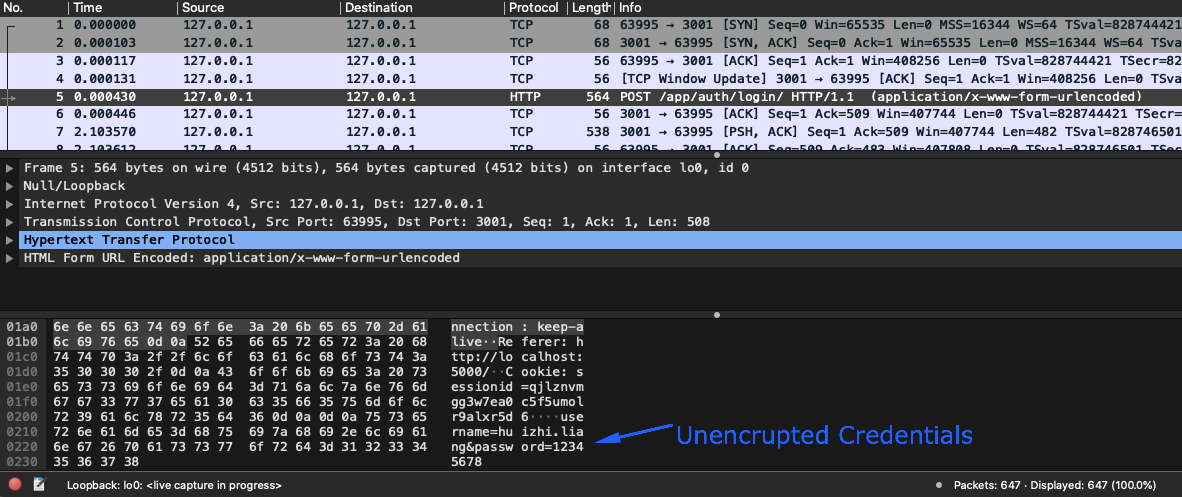
\includegraphics[scale=0.3]{figures/http}
				\fi
			\end{figure}
			\begin{figure}[H]
				\iftrue
				\caption{Ecrupted Credentials (HTTPS enabled)}
				\centering
				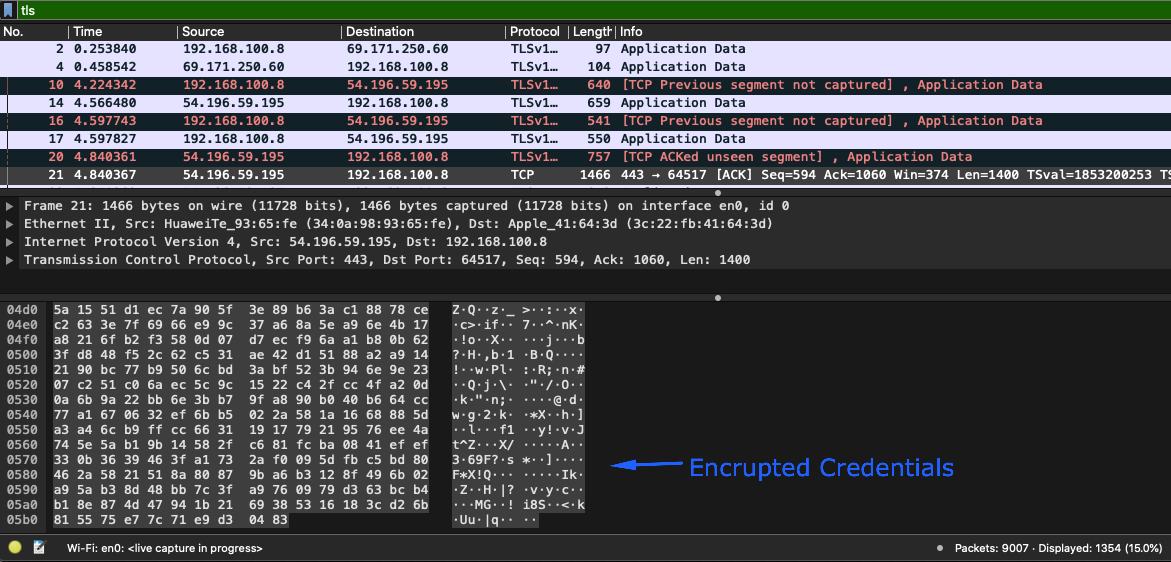
\includegraphics[scale=0.3]{figures/https}
				\fi
			\end{figure}
			Becomes evident that, by using HTTPS we increase our system security, as credentials and personal information are encrupted before sent over the
			internet.
		\subsection{RESTFull protocol}
			

    \chapter{The Backend}
\label{backend}
	\section{Introduction}
		\begin{figure}[H]
			\iftrue
			\caption{Backend Services}
			\centering
			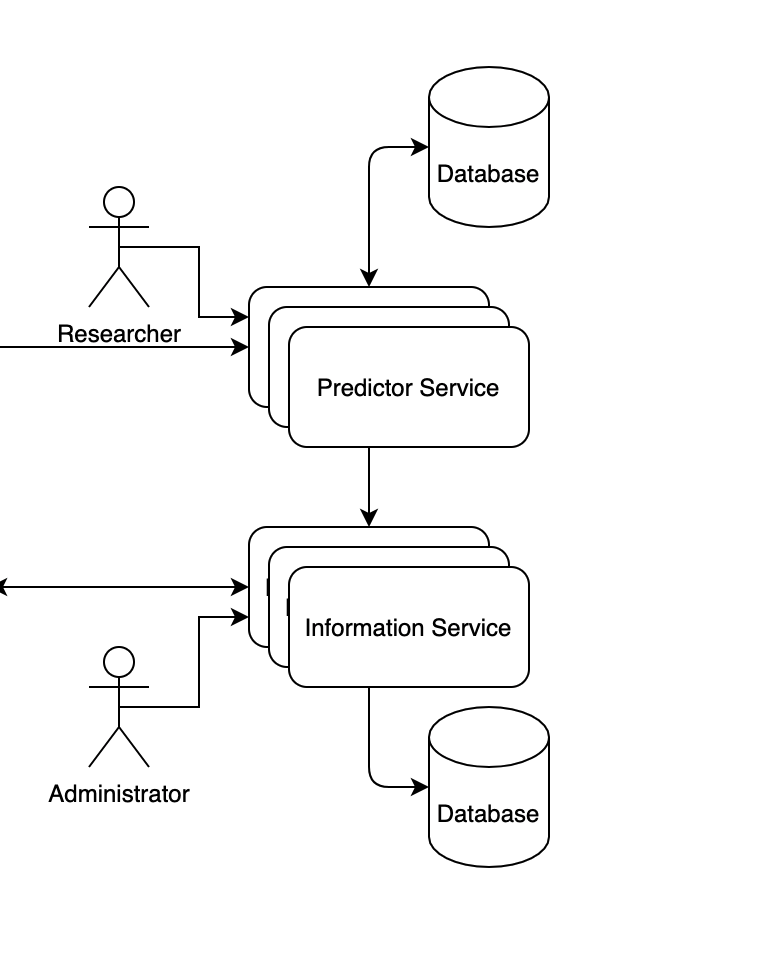
\includegraphics[scale=0.5]{figures/backend}
			\fi
		\end{figure}
		In this chapter we will cover extensively the inner workings of the backend services, namely the Information and the Prediction services
		We will go through their internal architectures as well as some key areas of interest.
	\section{Information Service}
		The Information Service(internally known as uortmc-infobe) is the service that handles the information of our entities, namely the
		patients, the scans, the end-users and their interconnections, additionally it handles authentication and includes the notification
		system, capable of notifying a given end-user for the completion of their tasks.\par
		\subsection{Technology Stack}
			The Information service uses a number of libraries to achieve its goals, the most important ones are listed below
			\begin{itemize}
				\item Django framework
				\item psycopg2 database driver
			\end{itemize}	
			\subsubsection{Django Framework}
				\label{django}
				Django is a free and open-source, python based web framework that uses the model-template-view(MTV) architecture pattern. 
				It is maintained by an american  501(c)(3) non-profit organisation called Django Software Foundation (DSF). Django offers 
				the code infastructure to develop RESTFul[\cite{restful-rfc7231}] microservices with ease, and its the backbone of both of our
				microservices
			\subsection{psycopg2 database driver}
				\label{psycopg2}
				psycopg2 is a famous postgres database driver for python. psycopg2 offers the interface for our postgres database connection, 
				implementing the server-client protocol behind the scenes.
		\subsection{Code Architecture}
			The Information service is designed to be a fully Object Oriented Entity[\cite{oop}].
			The architectural design of the Information Service can be seen below.\pagebreak
			\begin{figure}[H]
				\iftrue
				\caption{OOP Diagram}
				\centering
				 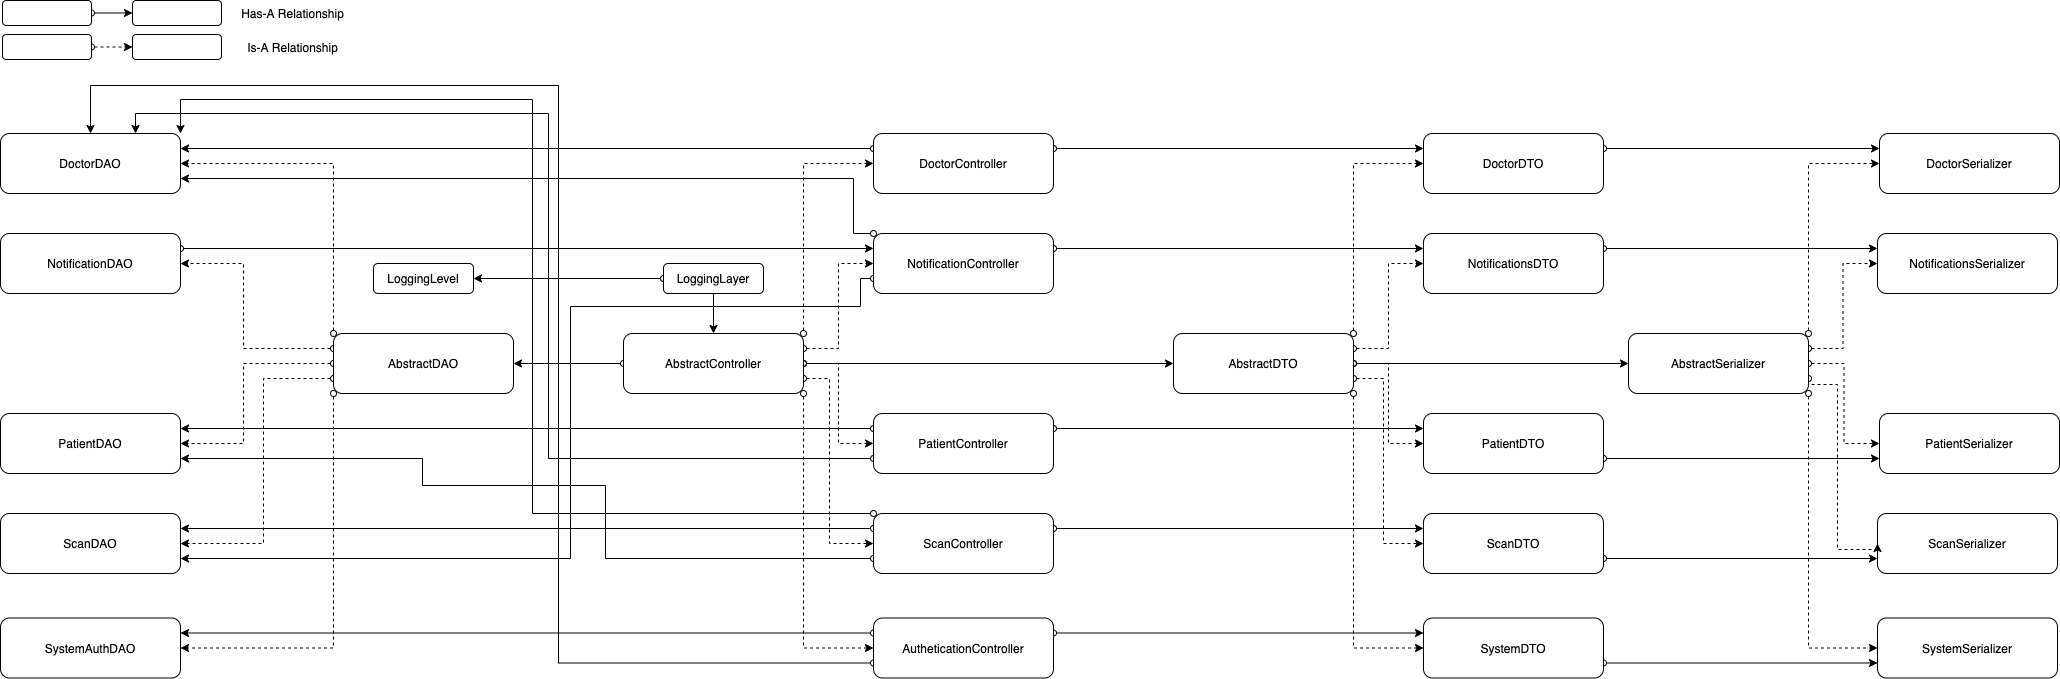
\includegraphics[angle=90,origin=c,scale=0.3]{figures/InformationServiceArchitecture}
				\fi
			\end{figure}\pagebreak
			The entrypoints for the requests, are the following classes
			\begin{itemize}
				\item \textbf{DoctorController}: This Class handles everything related to the Doctor Entity.
				\item \textbf{NotificationController} : This Class handles everything related to the Notification Entity.
				\item \textbf{PatientController} : This Class handles everything related to the Patient Entity.
				\item \textbf{ScanController} : This Class handles everything related to the Scan Entity.
				\item \textbf{AutheticationController} : This Class handles everything related to the Authentication service.
			\end{itemize}
			When a request is sent to the Information service, the proper Class is selected based on the request endpoint and details. 
			Then the respective class will use the rest of the classes services to perform the needed actions and respond to the request
			accordincly. A exhaustive list of the rest major classes are given below.
			\begin{center}
				\begin{tabular}{ |c|c| } 
					\hline
					DoctorDAO & Handles the SQL Queries of Doctor Entity \\
					NotificationDAO & Handles the SQL Queries of Notification Entity  \\\
					PatientDAO & Handles the SQL Queries of the Patient Entity\\
					ScanDAO & Handles the SQL Queries of the Scan Entity\\
					SystemAuthDAO & Handles the SQL Queries of the Authentication service\\
					AbstractDAO & Used to describe any DAO(Data Access Object) available\\
					LoggingLayer & Used by controllers to notify the operator in case of errors\\
					LoggingLevel &Used by LoggingLayer to describe the severity of an error\\
					AbstractController & Used to describe any controller available\\
					AbstractDTO & Used to describe any DTO(Data Transfer Object)'s available\\
					DoctorDTO & The responce objects for Doctor Entities\\
					NotificationsDTO & The responce objects for Notification Entities\\
					PatientDTO & The responce objects for Patient Entities\\
					ScanDTO & The responce objects for Scan Entities\\
					SystemDTO & The responce objects for Authentication Entities\\
					AbstractSerializer & Used to describe any serializer available\\
					DoctorSerializer & Used to convert Doctor DTO responce into JSON\\
					NotificationsSerializer & Used to convert Notification DTO responce into JSON\\
					ScanSerializer & Used to convert Scan DTO responce into JSON\\
					SystemSerializer & Used to convert SystemAuthDTO responce into JSON\\
					\hline
				\end{tabular}
			\end{center}
		\subsection{Database Medium}
			The Information Service uses an RDBMS(Relational Database Managment System)[\cite{friedrichsen_ruffolo_monk_starks_pratt_last_1995}] called Postgres. PostgreSQL is a open-source and 
			free relational database emphasizing on extensibility and SQL standard compliance. The relational diagram of the Information Service
			can be seen below.Additional information relating the E-R Diagram can be found in chapter \ref{entity-relation-analysis} \pagebreak
			\begin{figure}[H]
				\iftrue
				\caption{E-R Diagram}
				\centering
				\includegraphics[angle=90,origin=c,scale=0.8]{figures/InformationServiceDatabaseDiagram}
				\fi
			\end{figure}\pagebreak
	
	\section{Prediction Service}
		The Information Service(internally known as uortmc-taskbe) is the service that handles the prediction proccess ultrasound images, it has 
		also the responsibility of notifing the end-user when a task is completed, by calling the Information Service's Notification service 
		\subsection{Technology Stack}
		The Prediction service uses a number of libraries to achieve its goals, the most important ones are listed below
		\begin{itemize}
			\item Django framework (see paragraph \ref{django})
			\item psycopg2 database driver (see paragraph \ref{psycopg2})
			\item base64 decoders
			\item imghdr image
		\end{itemize}
		\subsection{Code Architecture}
		The Information service is designed to be a fully Object Oriented Entity[\cite{oop}].
		The architectural design of the Information Service can be seen below.\pagebreak
		\begin{figure}[H]
			\iftrue
			\caption{OOP Diagram}
			\centering
			\includegraphics[angle=90,origin=c,scale=0.3]{figures/InformationServiceArchitecture}
			\fi
		\end{figure}\pagebreak
		The entrypoints for the requests, are the following classes
		\begin{itemize}
			\item \textbf{DoctorController}: This Class handles everything related to the Doctor Entity.
			\item \textbf{NotificationController} : This Class handles everything related to the Notification Entity.
			\item \textbf{PatientController} : This Class handles everything related to the Patient Entity.
			\item \textbf{ScanController} : This Class handles everything related to the Scan Entity.
			\item \textbf{AutheticationController} : This Class handles everything related to the Authentication service.
		\end{itemize}
		When a request is sent to the Information service, the proper Class is selected based on the request endpoint and details. 
		Then the respective class will use the rest of the classes services to perform the needed actions and respond to the request
		accordincly. A exhaustive list of the rest major classes are given below.
		\begin{center}
			\begin{tabular}{ |c|c| } 
				\hline
				DoctorDAO & Handles the SQL Queries of Doctor Entity \\
				NotificationDAO & Handles the SQL Queries of Notification Entity  \\\
				PatientDAO & Handles the SQL Queries of the Patient Entity\\
				ScanDAO & Handles the SQL Queries of the Scan Entity\\
				SystemAuthDAO & Handles the SQL Queries of the Authentication service\\
				AbstractDAO & Used to describe any DAO(Data Access Object) available\\
				LoggingLayer & Used by controllers to notify the operator in case of errors\\
				LoggingLevel &Used by LoggingLayer to describe the severity of an error\\
				AbstractController & Used to describe any controller available\\
				AbstractDTO & Used to describe any DTO(Data Transfer Object)'s available\\
				DoctorDTO & The responce objects for Doctor Entities\\
				NotificationsDTO & The responce objects for Notification Entities\\
				PatientDTO & The responce objects for Patient Entities\\
				ScanDTO & The responce objects for Scan Entities\\
				SystemDTO & The responce objects for Authentication Entities\\
				AbstractSerializer & Used to describe any serializer available\\
				DoctorSerializer & Used to convert Doctor DTO responce into JSON\\
				NotificationsSerializer & Used to convert Notification DTO responce into JSON\\
				ScanSerializer & Used to convert Scan DTO responce into JSON\\
				SystemSerializer & Used to convert SystemAuthDTO responce into JSON\\
				\hline
			\end{tabular}
		\end{center}
		\subsection{Database Medium}
		The Information Service uses an RDBMS(Relational Database Managment System)[\cite{friedrichsen_ruffolo_monk_starks_pratt_last_1995}] called Postgres. PostgreSQL is a open-source and 
		free relational database emphasizing on extensibility and SQL standard compliance. The relational diagram of the Information Service
		can be seen below.Additional information relating the E-R Diagram can be found in chapter \ref{entity-relation-analysis} \pagebreak
		\begin{figure}[H]
			\iftrue
			\caption{E-R Diagram}
			\centering
			\includegraphics[angle=90,origin=c,scale=0.8]{figures/InformationServiceDatabaseDiagram}
			\fi
		\end{figure}\pagebreak
			
		
    \chapter{The Prediction Proccess}
\label{prediction-process}
	\section{Introduction}
		In this section, we will discuss the algorithms involved in the prediction process, a process running inside the Prediction Service, 
		and the libraries and the schematics of the predictors themselves.
	\section{Technology Stack}
		The prediction process uses several libraries to achieve its goals; the most important ones are listed below.
		\begin{itemize}
			\item Numpy linear algebra library.
			\item Scikit-learn machine learning library.
			\item torch and torchvision deep learning library.
		\end{itemize}
		\subsection{Numpy}+
			\label{numpy}
			Numpy is a python compatible library, adding support for matrices and multi-dimensional arrays, along with an 
			extesive set of routines, for linear algebra operations. We use Numpy for various image transformations, spatial 
			domain image filters and dataset handling
		\subsection{Scikit-learn}
			Scikit-learn is an open-source and free machine learning library compatible with python. Includes a rich 
			ecosystem of regression and clustering algorithms, including but not limited to random forests, vector machines, 
			gradient boosting k-means, and others. It is designed to interoperate with numerous Python numerical and scientific 
			libraries such as NumPy and SciPy.
		\subsection{pytorch and pytorchvision}
			PyTorch and pytorchvision are the python bindings of the famous torch library. Torch is a free and 
			open source deep learning and natural language processing library developed by Facebook's AI Research Lab.
	\section{Prediction Algorithms}
		In this section we will briefly discuss the two algorithms that our application currently supports, namely 
		\begin{itemize}
			\item C-Support Vector Machine, codenamed SVC v1.
			\item Residual Deep Neural Network, codenamed RESNet v18
		\end{itemize}
		\subsection{C-Support Vector Machine}
			Our first prediction algorithm, is a support vector machine[\cite{support-vector-machines}]. 
			A support vector machine is a supervised learning method that uses statistical learning frameworks[\cite{vapnik_2008}]
			to learn and classify binary datapoints, i.e., is a non-probabilistic binary linear classifier. The choice for the specific 
			classifier was based on its robustness and efficiency, especially when we have plenty of data points available. 
			\subsubsection{Prediction Process}
				The prediction process consists of 10 steps, those are.\pagebreak
				\begin{figure}[H]
					\iftrue
					\caption{SVC Prediction Process visualized}
					\centering
					\includegraphics[angle=90,origin=c,scale=0.7]{figures/svc-process}
					\fi
				\end{figure}\pagebreak
			\subsubsection{TDID Dataset}
				TDID (Thyroid Digital Image Database) is an open database of 400 360x560  thyroid ultrasound images, as well as with XML metadata 
				about these images, such as TIRADS classification[\cite{li_ma_cui_2018}] and region of interest(region of the nodule).
				We convert the TDID Dataset images and metadata to Numpy(paragraph \ref{numpy}) arrays in the first step of the process.
			\subsubsection{Image Filters}
				After the dataset has been loaded, we apply 2 simple spatial domain filters to every ultrasound image, the filters are
				\begin{itemize}
					\item DismissRGBChannels : converts the numpy-array representation of the image to grayscale, by converting the 
					3 RGB color channels to 1 Grayscale channel.
					\item Chop : Chops the scans unessesary areas, leaving the region of interest at the center.
				\end{itemize}
			\subsection{Dataset Shuffling}
				In this step, the dataset is shuffled to ensure that the algorithm will not overfit the given data in this run.
			\subsection{Dataset-Split}
				As required in every Hold-Out 80-20 training process, in this step the dataset is splitted in training and validation data,
				in a 80\%-20\% setup.
			\subsection{Train-Validate}
				After the shuffling part is complete, the SVC Model starts training. When the training is over, we calculate the confusion matrix
				and estimate the model accuracy.
			\subsection{Predict}
				After the training is complete, our model is ready to accept the end-users ultrasound image for prediction. In this step, we
				decode the image from its original base64 and JPEG encodings, and converting it into a numpy-array(paragraph\ref{numpy}).Finally
				the SVC can predict the classification of the image.
			\subsubsection{Model Performance}
				Our model has median accuracy rate of 72\% (100000 repeats), having the following hyperparameters
				\begin{itemize}
					\item gamma=0.001
					\item C=100
				\end{itemize}
		\subsection{Residual Deep Neural Network}
			To prove the application's ability to handle deep learning models, in agreement with my supervisor, Mrs. Huizhi Liang's 
			research team, we loaded an experimental prediction model to the application to measure the application's performance. 
			The deep learning model chosen is a Residual neural network. The application handled the more complex network successfully, 
			providing the following results after 10000 runs.
			\begin{itemize}
				\item Mean Responce Time(MRT) : 3.62s
				\item Mean Memory Used : 32.7mb
				\item Mean Swap Used : 0mb
			\end{itemize}
			Those results fullfil the requirement criteria (paragraph \ref{non-functional-requirements}).
			
			
		


    \chapter{CICD-Versioning-Deployment}
\label{cicd-versioning-deployment}

...
\section{...}
....


\section{...}
...


\subsection{...}


\section{Summary}
...


			
			
			
			
			
			
			
		
	




    \chapter{Starting The Application Locally}
\label{start-stop-guide}
	\section{Introduction}
		In this section, we will start our exploration of the application and its features. As the nature of the requirements of this
		the system is complicated. Unavoidably the system will be complex as well. Taking this into consideration, we will follow a natural top-to-bottom
		approach explaining its internals, starting as end-users and seeing the system as a black box. In this section, we will analyze its 
		functionality from the user's perspective. This section may also serve as an instruction manual for the end-user as it contains everything needed
		for an inexperienced user to start working with the software.
	\section{Login and Authentication}
		\begin{figure}[H]
			\iftrue
			\centering
			\caption{Login Screen}
			\includegraphics[scale=0.3]{figures/login}
			\fi
		\end{figure}
		The login screen is the first screen that our end-users will encounter. Here a username and a password is required to be given by the 
		user to log in. The Credentials of the user remain encrypted during the process of login, as the system utilizes an HTTPS[\cite{rfc2818}] 
		protocol for its connection, this is essential for the first non-functional requirement about security (see \ref{non-functional-requirements}).
		The username and the password may be requested by the system administrator or the NOC\footnote{Network Operations Center} of the hospital.
	\section{Home}
		\begin{figure}[H]
			\iftrue
			\centering
			\caption{Home Screen}
			\includegraphics[scale=0.3]{figures/home}
			\fi
		\end{figure}
		After the login process is completed. The user encounters the 'home screen. From here, it is possible to navigate to the features of the software
		as well as learn about how the software can be utilized through detailed guides and videos. The UI/UX\footnote{User Interface-User Expieriance} 
		has been designed to be as user-friendly as possible. Some areas of interest are given below.
		\begin{center}
			\begin{tabular}{ |c|c| } 
				\hline
				Action bar & The Actions that can be performed using the software can be accesed from here.\\
				Navigation bar & General information and notification bar. \\
				\hline
			\end{tabular}
		\end{center}
	\section{Navigation bar}
		In this section, we will briefly look at the options under the Navigation bar.
		\subsection{Profile}
			\begin{figure}[H]
				\iftrue
				\centering
				\caption{Profile}
				\includegraphics[scale=0.3]{figures/profile}
				\fi
			\end{figure}
			In the profile section, the user can see its associated information, saved on the registration date. 
			The information for security reasons cannot be altered by the user itself, but only after a request to 
			the system administrator or NOC\footnote{Network Operations Center}.
		\subsection{Notifications}
			\begin{figure}[H]
				\iftrue
				\centering
				\caption{Notifications}
				\includegraphics[scale=0.3]{figures/notifications}
				\fi
			\end{figure}
			In the notification section, helpful information about events that may interest the end-user can be found, 
			such as the fact that uploaded scan results are ready to view. 
		\subsection{About}
			\begin{figure}[H]
				\iftrue
				\centering
				\caption{About}
				\includegraphics[scale=0.3]{figures/about}
				\fi
			\end{figure}
			From here, a user may found helpful information about the software, such as the current version.
	\section{Action Bar}
		In this section, we will briefly look at the options under the Action Bar.
		\subsection{My Patients}
			\begin{figure}[H]
				\iftrue
				\centering
				\caption{Patients List}
				\includegraphics[scale=0.3]{figures/mypatients}
				\fi
			\end{figure}
			This page will show us a list of the currently registered patients. Each end-user(doctor) may only see its 
			patients and not others. The end-user can search the list based on NiNo[\cite{nino-format}] of the given 
			patient for convenience. The end-user can also view the details of a given patient and record various 
			notes/comments for that patient by clicking the 'Details' button on his selected patient, as seen below. 
			Finally, clicking the button 'View Scans' can see the specific patient history of uploaded scans.
			\begin{figure}[H]
				\iftrue
				\centering
				\caption{Patient Details}
				\includegraphics[scale=0.3]{figures/mypatients2}
				\fi
			\end{figure}
		\subsection{New Patient}
			\begin{figure}[H]
				\iftrue
				\centering
				\caption{New Patient}
				\includegraphics[scale=0.3]{figures/newpatient}
				\fi
			\end{figure}
			By clicking the 'New Patient' action on Action Bar, the user can register a new patient on the system. The following conditions need to 
			be met for the operation to be successful.
			\begin{itemize}
				\item First name length should be more than 2 characters, encoded as UTF-8[\cite{rfc3629}]
				\item Last name length should be more than 2 characters, encoded as UTF-8[\cite{rfc3629}]
				\item NiNo should be at standard format [\cite{nino-format}], encoded as UTF-8[\cite{rfc3629}]
			\end{itemize}
			Failing to fulfill these constraints should lead to an error, as shown below.
			\begin{figure}[H]
				\iftrue
				\centering
					\caption{New Patient Error}
				\includegraphics[scale=0.3]{figures/newpatient-error}
				\fi
			\end{figure}
		\subsection{My Scans}
			\begin{figure}[H]
				\iftrue
				\centering
				\caption{My Scans}
				\includegraphics[scale=0.3]{figures/myscans}
				\fi
			\end{figure}
			'MyScans' are a complete list with all submitted scans for a given end-user. 
			The user can search for the scans of a specific patient by using the search box and viewing the 
			scan results (if a given scan is complete) by clicking the 'Details' button of the scan in question.
			\begin{figure}[H]
				\iftrue
				\centering
				\caption{Scan results}
				\includegraphics[scale=0.3]{figures/myscans-details}
				\fi
			\end{figure}
		\subsection{New Scan}
			\begin{figure}[H]
				\iftrue
				\centering
				\caption{New Scan}
				\includegraphics[scale=0.3]{figures/newscan}
				\fi
			\end{figure}
			By clicking the 'New Scan' action, the user is redirected into the scan submission form. Here it is possible to 
			submit a new ultrasound image for a given patient.The user can also select the algorithm for performing the 
			classification (see \ref{prediction-service}). The operation to be completed should meet the following criteria.
			\begin{itemize}
				\item Patients Nino should be in standard format[\cite{nino-format}] and encoded as UTF-8[\cite{rfc3629}]
				\item Scan Image should be a ISO/IEC 10918-1/JPEG[\cite{jpeg-iso10918-1}] format with 360x560 resolution. The image name
				should be encoded as UTF-8[\cite{rfc3629}]
			\end{itemize}
			Failing to fulfill these constraints should lead to an error, as shown below.
			\begin{figure}[H]
				\iftrue
				\centering
				\caption{Invalig image format (PNG) error}
				\includegraphics[scale=0.3]{figures/newscan-error}
				\fi
			\end{figure}
			
			
			
			
			
			
			
		
	




    \chapter{Discussion, Conclusion and Future work}
\label{ch:lit_rev}
	\section{Introduction}
		It is for certain that this first iteration is not perfect by any means, much work need to be done for this project to become 
		a contributing tool for the academic community, but the results are iitial results are promising. After working closely with
		my supervisor, Mrs Liang, We started disqussing the possibility of continuing the develepoment of this project if sufficient
		funding is found, if this is the case then this tool has the capability to speed up the Thyroid nodule classification research even
		more.
	\section{Future work}
		There are multiple areas that we can focus on to improve the application and its performance, some proposed ideas are presented below
		\subsection{Improving the SVC Prediction Model}
			There are multiple chances for improvement when comes to the prediction model, for improving its accuracy results. A proposed
			area of improvement is to, instead of binary classifing the given ultrasound image, to also find the exact thuroid nodule borders
			within the image, by taking advantage the additional metadata given by the TDID dataset.
		\subsection{Multiple prediction models and vote system}
			A different idea that was proposed, is the utilisation of multiple prediction models, and the aggregation into a single view, increasing
			the accuracy results, by the prediction answer of every algorithm, and based on an weighted system of voting, to determine the actual
			prediction.
		\subsection{Application monitoring using Graphana}
			A proposal coming from the fact that the application does not have any monitoring capability at the moment. By adding monitoring
			we can have real-time metrics about the applications performance and status, This will be a great tool for the administrator operator as it
			will provide the capability to react in sudden surges in demand, or possible errors quicker.
		
		
...



    \chapter{Reflection}

	Thyroid nodule classification is a challenging branch of machine learning, having deep roots in Artificial intelligence, 
	deep learning, statistical analysis, Image Analysis, and mathematics. It was a great challenge and a massive opportunity 
	for me as I had to catch up with all those diverse topics as well as to combine them with my computer science knowledge, 
	as well as to engage with the academic community, and work closely with my supervisor's research team for a whole year. 
	The result was rewarding as I successfully cooperated with the research team, learned the necessary material, and developed
	a scientific application with actual applications for the academic community. It was an excellent experience that gave me 
	technical knowledge and management and communication skills that I needed for my future. My personal opinion was that it 
	was a complete 'real-world' experience that gave me everything I need for success.
...



    
    
    % -------------------------------------------------------------------
    % References  -  Harvard Style was used in this report
    % -------------------------------------------------------------------
    \bibliographystyle{agsm} % Harvard Style 
    
    \bibliography{references}  %  Patashnik, O. (1988), BibTEXing. Documentation for general BibTEX users.
    	
    % -------------------------------------------------------------------
    % Appendices
    % -------------------------------------------------------------------

    
\end{document}
